% Options for packages loaded elsewhere
\PassOptionsToPackage{unicode}{hyperref}
\PassOptionsToPackage{hyphens}{url}
%
\documentclass[
]{book}
\usepackage{amsmath,amssymb}
\usepackage{lmodern}
\usepackage{ifxetex,ifluatex}
\ifnum 0\ifxetex 1\fi\ifluatex 1\fi=0 % if pdftex
  \usepackage[T1]{fontenc}
  \usepackage[utf8]{inputenc}
  \usepackage{textcomp} % provide euro and other symbols
\else % if luatex or xetex
  \usepackage{unicode-math}
  \defaultfontfeatures{Scale=MatchLowercase}
  \defaultfontfeatures[\rmfamily]{Ligatures=TeX,Scale=1}
\fi
% Use upquote if available, for straight quotes in verbatim environments
\IfFileExists{upquote.sty}{\usepackage{upquote}}{}
\IfFileExists{microtype.sty}{% use microtype if available
  \usepackage[]{microtype}
  \UseMicrotypeSet[protrusion]{basicmath} % disable protrusion for tt fonts
}{}
\makeatletter
\@ifundefined{KOMAClassName}{% if non-KOMA class
  \IfFileExists{parskip.sty}{%
    \usepackage{parskip}
  }{% else
    \setlength{\parindent}{0pt}
    \setlength{\parskip}{6pt plus 2pt minus 1pt}}
}{% if KOMA class
  \KOMAoptions{parskip=half}}
\makeatother
\usepackage{xcolor}
\IfFileExists{xurl.sty}{\usepackage{xurl}}{} % add URL line breaks if available
\IfFileExists{bookmark.sty}{\usepackage{bookmark}}{\usepackage{hyperref}}
\hypersetup{
  pdftitle={Finance},
  pdfauthor={Dyrehaugen Web Notebook},
  hidelinks,
  pdfcreator={LaTeX via pandoc}}
\urlstyle{same} % disable monospaced font for URLs
\usepackage{longtable,booktabs,array}
\usepackage{calc} % for calculating minipage widths
% Correct order of tables after \paragraph or \subparagraph
\usepackage{etoolbox}
\makeatletter
\patchcmd\longtable{\par}{\if@noskipsec\mbox{}\fi\par}{}{}
\makeatother
% Allow footnotes in longtable head/foot
\IfFileExists{footnotehyper.sty}{\usepackage{footnotehyper}}{\usepackage{footnote}}
\makesavenoteenv{longtable}
\usepackage{graphicx}
\makeatletter
\def\maxwidth{\ifdim\Gin@nat@width>\linewidth\linewidth\else\Gin@nat@width\fi}
\def\maxheight{\ifdim\Gin@nat@height>\textheight\textheight\else\Gin@nat@height\fi}
\makeatother
% Scale images if necessary, so that they will not overflow the page
% margins by default, and it is still possible to overwrite the defaults
% using explicit options in \includegraphics[width, height, ...]{}
\setkeys{Gin}{width=\maxwidth,height=\maxheight,keepaspectratio}
% Set default figure placement to htbp
\makeatletter
\def\fps@figure{htbp}
\makeatother
\setlength{\emergencystretch}{3em} % prevent overfull lines
\providecommand{\tightlist}{%
  \setlength{\itemsep}{0pt}\setlength{\parskip}{0pt}}
\setcounter{secnumdepth}{5}
\usepackage{booktabs}
\usepackage{amsthm}
\makeatletter
\def\thm@space@setup{%
  \thm@preskip=8pt plus 2pt minus 4pt
  \thm@postskip=\thm@preskip
}
\makeatother

\renewcommand\chaptername{}
\ifluatex
  \usepackage{selnolig}  % disable illegal ligatures
\fi
\usepackage[]{natbib}
\bibliographystyle{apalike}

\title{Finance}
\author{Dyrehaugen Web Notebook}
\date{2021-04-26}

\begin{document}
\maketitle

{
\setcounter{tocdepth}{1}
\tableofcontents
}
\hypertarget{finance}{%
\chapter{Finance}\label{finance}}


\includegraphics{fig/zelda.jpg}

\hypertarget{finance-1}{%
\chapter{Finance}\label{finance-1}}

\hypertarget{money}{%
\section{Money}\label{money}}

\begin{quote}
Money is the alienated essence of man's labour and life; and this alien essence dominates him as he worships it. (Karl Marx)
\end{quote}

\hypertarget{institutional-investors}{%
\subsection{Institutional Investors}\label{institutional-investors}}

\hypertarget{esg-2.0}{%
\subsubsection{ESG 2.0}\label{esg-2.0}}

\emph{Segal}

\textbf{How Institutional Investors Encourage Corporations Bad Behavior}

Wittingly or unwittingly, pensions and endowments' investment strategies aid and abet activities that make the financial system more fragile.

The growing scale of institutions and the large amounts of money they need to deploy into high-risk investments is leading to consolidation among asset managers, higher global debt levels, short-term corporate behavior, and market instability.

Institutions' investment strategies are in conflict with environmental, social, and governance goals to which they are increasingly committing.

Pension funds, insurance companies, sovereign wealth funds and others need to deploy large amounts of capital efficiently because they themselves are so big.

Institutions' only option in many cases is to put billions of dollars to work in the largest public and private companies, Rothenberg explained. That results in companies, for example, taking on unsustainable amounts of debt.

There are incentives to layer on debt, much of which is supplied by capital markets and the shadow banking sector.

Ironically, institutional investors want to integrate ESG into their process, but they also contribute to corporate consolidation and huge debt burdens. Institutional investors are essentially contributing to some of their own problems in the way they allocate capital to leveraged loans, high-yield loans, collateralized loan obligations
and other higher risk products.

All of this adds to global systemic risks.
Unchecked increases in corporate debt result in increased systematic market risk that boomerangs back to investors and their portfolios
Existing approaches like Modern Portfolio Theory and ESG or impact investing frameworks don't focus on these potentially negative effects.

Perversely, as major central banks globally respond to the current crisis with rock bottom interest rates and new rounds of quantitative easing (QE), investors and companies are further incentivized to increase their exposure to high-risk debt and inflated asset valuations --- a situation that leaves society and markets vulnerable to a rise in interest rates or other unplanned challenges

\href{https://www.institutionalinvestor.com/article/b1r9js87jhyn8s/How-Institutional-Investors-Encourage-Corporations-Bad-Behavior}{Segal - Comment - Instititional Investor}

\emph{Rothenburg}

Many of our existing ESG and impact investing frameworks focus on issues at the
portfolio company level, but they do not take into account potential negative
impacts from capital structures and investors' influence in shaping them.
Asset allocation strategies can be in conflict with ESG objectives.

The conflict materializes in various interconnected ways, particularly from
institutional investors' role in increasing global debt levels and
fund manager and corporate consolidation.

For long-term, diversified institutional investors, or ``Universal Owners''
of the market, these dynamics eventually translate into lower financial returns.
For workers and communities, these dynamics translate into
greater precarity and inequality.

Potential solutions focus on diversifying asset allocation to
more regenerative investment structures and asset classes, building an
enabling environment through adjustments to team incentive structures, performance reviews,
benchmarking and valuation methodologies, and field-building.

Over the past decades, institutional investors have migrated up
the risk-return spectrum to asset classes with higher yields.
Investor allocations to private equity (PE), venture capital (VC), private debt (PD),
high yield bonds (HYBs), leveraged loans (LLs), and
collateralized loan obligations (CLOs), for instance,
have been growing steadily in response to a number of trends.
\emph{While such shifts in asset allocation may suit near-term goals,
such as meeting actuarial targets, this institutional allocation to higher risk asset
classes has also meant increased global debt burdens, corporate and
fund manager consolidation, and risk across capital structures,
resulting in fragility for companies, the real economy, and the stability of
financial markets.
The resulting risks are therefore shared not only by investors,
but also governments,workers, and communities alike.}

To optimize leverage ratios, companies may prioritize debt servicing or distributions to investors at the
expense of worker payrolls and benefits. Infrastructure and social infrastructure investments --- such as
power, water, roads, hospitals, nursing homes, housing, and cybersecurity --- might be structured in
such a way that provides access to end-users at unaffordable prices, or of poor quality, in order to meet
investor return expectations and therefore attract capital. Weak capital structures increase the risk of
restructurings or bankruptcies that are detrimental for stakeholders, such as workers. Stakeholders have
increasingly raised concerns about high leverage, coined ``financial engineering,'' particularly in the PE
asset class, for such reasons. 5 Yet studies produced over the past decades, inspired by PE, praise the
discipline of debt, and due to a number of additional factors, high leverage ratios are no longer confined
to the PE asset class and are prolific across public equity markets, as well.

In practice, the negative impacts of weak capital structures are typically being addressed piecemeal
through company-by-company interventions that focus on corporate operations, like a game of whack-
a-mole; but key roots of the problem --- the investment structures themselves --- are left unaddressed.

The unintended negative consequences of highly levered investments have been underexplored when it
comes to ESG and impact investing frameworks and practice. Matters relating to investment structures,
capital structures, leverage ratios, earnings calculations, valuation methodologies, benchmarking
approaches, and resulting asset allocation and portfolio construction are not typically within the realm
of ESG-related responsibilities.

Too much leverage is dangerous for all stakeholders.
While leverage looks like a neutral, bilateral accelerant, it
actually reduces financial resiliency at the very times when it might be most needed.

Systemic inequality has been shown to result in economic decline.

Neither Modern Portfolio Theory (MPT) nor ESG or impact investing frameworks
currently include a focus on potential negative impacts stemming from
investment structures.

Corporate debt burdens and leverage ratios are historically high, covenants are light, and
defaults and bankruptcies are being held at bay by government support
(e.g.~through fiscal and monetary policy) -- which is also funded by debt,
though at the sovereign level.

Corporate funding dynamics have changed since the Global Financial Crisis
(GFC), when banks came under heavy regulation that caused them to
restrict lending to smaller clients.
Capital markets, or the Non-bank Financial Intermediary
(``NBFI'' or ``Shadow Banking'') sector, has stepped in to fill this void.

The financial assets of the NBFI sector amounted to \$200.2 trillion in 2019,
accounting for nearly half of the global financial system in 2019, up from 42\%
in 2008

\emph{How Did We Get Here?}

For the past two decades, institutional asset owners have significantly shifted their overall asset
allocation strategy. Private markets -- including PE, PD, VC, infrastructure, and real estate - as well as LLs,
CLOs, and HYBs, have become much larger percentages of overall portfolios. There are a number of
reasons for these changes, including, but not limited to, ongoing declines in interest rates by major
global central banks, dynamics related to funding ratios of institutional investors such as pension funds,
growing interest in the illiquidity premium of private markets, benchmarking practices, investor
dissatisfaction with public markets, and increased opportunity for NBFIs to provide financing following
banking regulations resulting from the GFC. 16 Private capital assets under management (AUM) in 2019
was approximately US\$6.5 trillion, an increase of over US\$4 trillion over the past ten years.

\emph{Private Equity (PE)}

Investor demand is now so high for PE that many are concerned that the asset class is becoming crowded with capital.

Consolidated capital flows stems from the institutionalization of capital.
Markets have evolved from being dominated by individual investors to
having a large presence of institutional investors.
Institutional investors now hold over 40 percent of
global market capitalization of listed companies.

Institutional investors have sizable portfolios and must invest billions
if not trillions of dollars.
With such large chunks of capital to put to work,
they often find it challenging to invest in smaller fund managers,
smaller companies, and niche investment strategies due to a number of factors,
such as transaction costs.

Even when small deals perform well, which data suggests that they often do,
they are hard to justify because they do not meaningfully move the needle
in terms of overall portfolio returns.

A well-documented negative impact of consolidated capital flows to larger
fund managers is that
smaller, emerging, and innovative fund managers can be starved of capital.

\emph{Institutionalization of Capital}

The consolidation of capital among institutional investors is a double-edged sword. On the one hand,
institutions offer individual investors professional money management with multi-disciplinary staff and
robust internal infrastructure capable of constructing well-diversified portfolios. Size and scale can also allow
large allocators to influence corporate governance of portfolio companies, as well as negotiate more
attractive terms with fund managers. It is arguable that fees overall are reduced through these dynamics, and
strong ESG practices can be better advocated for. On the other hand, since large institutions need to put
significant amounts of capital to work, they often allocate to the largest managers and companies, thereby
resulting in consolidation of power, profit, influence, and opportunity among a shrinking pool of asset
managers and companies. 53 In order for large institutional investors to act as responsible Universal Owners
and effectively manage systematic risk, it will be critical for them to evaluate their asset allocation practices
for unintended negative consequences that not only impact the real economy, but also markets and their
long-term portfolios.

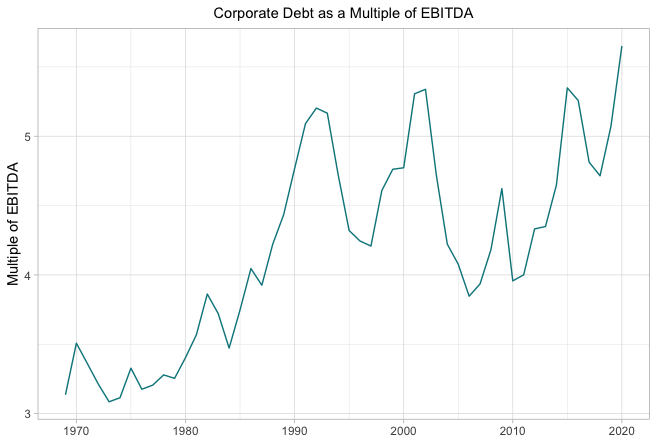
\includegraphics{fig/corporate_debt_ebitda.png}

This high-risk debt is not limited to private companies. A recent Forbes article highlights how, ``some of
the biggest firms in the United States\ldots{} have binged on low interest debt. Most of them borrowed more
than they needed, often returning it to shareholders in the form of buybacks and dividends. They also
went on acquisition sprees.''

From the corporate perspective, historically cheap credit due to low interest rates is attractive,
particularly when combined with the current tax deductibility of interest expense, studies suggesting
that highly leveraged capital structures do not negatively impact stock prices, and arguments that debt
adds discipline to corporate management. Yet debt and common uses of funds can increase risk for
other stakeholders. M\&A has been shown to contribute to corporate consolidation which can stifle
SMEs, innovation, suppliers, the quality and affordability of goods and services, labor's bargaining
power, and diversification for institutional investors. There is significant literature that explores
negative impacts of share buybacks in public companies, given the links with high executive
compensation and that cash paid to executives and shareholders can deter from reinvestment in the
company, the quality of goods and services, and the workforce. In PE-backed companies, high leverage
from acquisitions and dividend recapitalizations can push companies to cut costs related to quality jobs
and jeopardize the quality and affordability of goods and services.

As central banks around the world doubled down on low interest rates and QE, investors responded by
increasing portfolio allocation to higher risk and yielding asset classes.

The combination of QE and low interest rates with corporate consolidation and high
inequality may well be creating challenges to long-term economic growth,
as well as introducing
potential drivers of instability for aggregate demand.

\href{https://papers.ssrn.com/sol3/papers.cfm?abstract_id=3820316}{Rothenberg (2021) ESG 2.0 - Measuring \& Managing Investor Risks Beyond the Enterprise-level}
\href{Rothenberg_2021_ESG2.pdf}{(pdf)}

\hypertarget{central-banks}{%
\section{Central Banks}\label{central-banks}}

In managing our economy with disembedded measures of wealth,
the world's central bankers are effectively agents of the sustainability crisis. They may not
wish to be unsustainable by personal inclination, but they certainly are by professional
obligation because of how they are duty-bound to act.
An entirely foreseeable response to the climate emergency is that people in wealthier
countries may choose to pare back their consumption of non-essentials. Certainly, not
everyone has the luxury to do this, but the obvious solution of ``buying less stuff'' has become
an articulated idea in wealthy countries. ``Flight shaming'' and ``consumption shaming'' are new
memes. Articles in multiple UK newspapers have challenged readers to see if they can go a
year without buying any new clothes, contravening the media's normal practice of generally
trying to coax the economy along. (It buoys the advertising revenue).
Such behaviours would amount to a direct hit on GDP in developed countries, where personal
consumption can represent two-thirds of the total. Critically, any such reduction in
consumption will likely show up as a deflationary decline in economic activity that the world's
central banks are on hair-trigger alert to prevent. The large and powerful financial
bureaucracy stands ready to provide immediate stimulus to any perceived flagging of
measured economic activity.
Hence, the arrangement most populations in the world currently live under is that should they
collectively choose to buy less, more money will be printed until they have changed their
mind. Effectively, our exhausted ecosystem is gasping for a lull in measured economic activity
that our financial authorities are pledged to never let happen.

\href{pdf/Austin_2021_Pigou_\%20and_the_dropped_stitch_of_economics_RWER95.pdf}{Duncan Austin: Pigou and the dropped stitch of economics RWER95 (pdf)}

\hypertarget{central-bank-independence}{%
\subsubsection{Central Bank Independence}\label{central-bank-independence}}

\textbf{Market Neutrality}

\emph{Klooster Abstract}

Monetary policy operations in corporate security markets confront central
banks with choices that are traditionally perceived to be the prerogative of
governments. This article investigates how central bankers legitimise
corporate security purchases through a comparative study of the
European Central Bank (ECB) and the Swiss National Bank (SNB). As we
show, central bankers downplay the novelty of corporate security
purchases by relying on familiar pre-crisis justifications of Central Bank
Independence. Citing an ideal of `market neutrality', central banks
present corporate security purchases as pursuing a narrow objective of
price stability and obfuscate their distributive consequences. In this way,
central bankers depoliticise corporate security purchases: they reduce
the potential for choice, collective agency, and deliberation concerning
both the pursuit of corporate security purchases and the choices made
in implementing these policies. We also describe the undesirable
democratic, social and environmental dimensions of these practices,
which we propose to address through enhanced democratic
accountability.

\emph{Klooster Memo}

The past decades saw central banks acquire considerable independence from democratic institutions
(McNamara 2002, Singleton 2010). Governments justified their decision to delegate monetary policy
by relying on a narrow conception of monetary policy. This conception focuses on the setting of short
term interest rates to achieve a long-term objective of stable price levels. A crucial element in the
justification of central bank independence is the idea that monetary policy is an apolitical, technical
area of policymaking (Marcussen 2009). The loss of democratic control that results from the creation
of an independent central bank was also thought to be minimal, because distributive choices would
remain with elected governments, who both decided on the central bank mandate and retained the
use of fiscal instruments to achieve their distributive objectives. In this way, governments depoliticised
monetary policy in the sense of reducing the potential for choice, collective agency, and deliberation
around the use of monetary policy

The Global Financial Crisis (GFC) led central bankers to move far beyond the narrow task assigned
to them under the traditional justification of Central Bank Independence (CBI)
To rescue a global financial system on the brink of collapse, central bankers assumed new roles as lenders and market makers of last resort.

Central bankers, meanwhile, are openly concerned that the use of unconventional tools threatens
their independence.
When independent regulatory agencies extend their power, political authorities often seek to regain
control.
Central bankers, accordingly, try to counteract repoliticisation and these efforts
shape their policies.

To investigate the simultaneously occurring processes of politicisation and depoliticisation
we investigate how central bankers relate to the political dimensions of their
new unconventional policies.

\href{https://www.tandfonline.com/doi/epub/10.1080/13563467.2019.1657077?needAccess=true}{Klooster (2021) The Myth of Market Neutrality}
\href{pdf/Klooster_2021_Myth_of_Market_Neutrality.pdf}{(pdf)}

The new exogenous money is exogenous transition shocks in the climate change debate.
Fortunately, Bank of England cannot hide behind that rock because of their new climate mandate.

Remember, Mark Carney's `tragedy of the horizons' speech identified two main risks of climate crisis:
- physical risks (climate events)
- transition risks - from green policies to accelerate transition to low-carbon

Now, central banks are confronted with an unpleasant conundrum that reveals the deeply political nature of their operations:
greening monetary policy (collateral, unconventional bond purchases) means endogenous transition risks

So, in a have your cake and eat it moment, there is a growing tendency in central bank communities to pretend that all transition risks come from the fiscal side (carbon pricing)

It wouldn't be surprising to find the exogenous transition shocks approach in the ECB's monetary policy strategy review, despite \citet{Lagarde}
and other's recognition that central banks cannot longer hide behind the `market neutrality' argument.

\href{https://twitter.com/DanielaGabor/status/1384837864412917765}{Gabor (Twitter)}

\hypertarget{financial-stability}{%
\subsection{Financial Stability}\label{financial-stability}}

\hypertarget{climate-risk}{%
\subsubsection{Climate Risk}\label{climate-risk}}

\hypertarget{bis-recommendations}{%
\paragraph{BIS Recommendations}\label{bis-recommendations}}

This report provides an overview of conceptual issues related to climate-related financial risk
measurement and methodologies, as well as practical implementation by banks and supervisors.

The report contains five key findings:
First, climate-related financial risks have unique features, necessitating granular and
forward-looking measurement methodologies.

Second, to date, measurement of climate-related financial risks by banks and supervisors
has centred on mapping near-term transition risk drivers into counterparty and portfolio exposures.

Third, banks and supervisors have predominantly focused on assessing credit risk, as they
advance in applying methods to translate climate-related exposures into categories of financial risk.

Fourth, while banks and supervisors remain at an early stage of translating climate-related
risks into robustly quantifiable financial risk, work continues to gather pace

Fifth, key areas for future analytical exploration relate to measurement gaps in data and
risk classification methods, as well as methodologies suitable for assessing long-term climate
phenomena not always of a standard nature.

\href{https://www.bis.org/bcbs/publ/d518.htm}{BIS (2021) Climate Risk}
\href{pdf/BIS_2021_Climate_Risk.pdf}{(pdf)}

\hypertarget{index-providers}{%
\section{Index Providers}\label{index-providers}}

\emph{Fitchner}

A silent revolution is happening in investing. It is a paradigm shift that will have a profound impact on corporations, countries and pressing issues like climate change.
A silent revolution is happening in investing. It is a paradigm shift that will have a profound impact on corporations, countries and pressing issues like climate change.
In 2019 there was a watershed in the history of finance. In the United States, the total value of actively managed funds was surpassed by passive funds. Globally, passive funds crossed US\$10 trillion (£7.7 trillion), a five-fold increase from US\$2 trillion in 2007.

This seemingly unstoppable ascent has two main consequences.

First, corporate ownership has become concentrated in the hands of the ``big three'' passive asset managers: BlackRock, Vanguard and State Street. They are already the largest owners of corporate America.

The second consequence relates to the companies that provide the indices that these passive funds follow. When investors buy index funds, they effectively delegate their investment decisions to these providers. Three dominant providers have become increasingly powerful: MSCI, FTSE Russell and S\&P Dow Jones Indices.

A silent revolution is happening in investing. It is a paradigm shift that will have a profound impact on corporations, countries and pressing issues like climate change. Yet most people are not even aware of it.

In a traditional investment fund, the decisions about where to invest the capital of the investors are taken by fund managers. They decide whether to buy shares in firms like Saudi Aramco or Exxon. They decide whether to invest in environmentally harmful businesses like coal.

Yet there has been a steady shift away from these actively managed funds towards passive or index funds. Instead of depending on a fund manager, passive funds simply track indices -- for example, an S\&P 500 tracker fund would buy shares in every company in the S\&P 500 in order to mirror its overall performance. One of the great attractions of such funds is that their fees are dramatically lower than the alternative.

In 2019 there was a watershed in the history of finance. In the United States, the total value of actively managed funds was surpassed by passive funds. Globally, passive funds crossed US\$10 trillion (£7.7 trillion), a five-fold increase from US\$2 trillion in 2007.
¿Le gusta lo que lee? ¿Quiere más?

This seemingly unstoppable ascent has two main consequences. First, corporate ownership has become concentrated in the hands of the ``big three'' passive asset managers: BlackRock, Vanguard and State Street. They are already the largest owners of corporate America.

The second consequence relates to the companies that provide the indices that these passive funds follow. When investors buy index funds, they effectively delegate their investment decisions to these providers. Three dominant providers have become increasingly powerful: MSCI, FTSE Russell and S\&P Dow Jones Indices.

With trillions of dollars migrating to passive funds, the role of index providers has been transformed.

In the past, index providers only supplied information to financial markets. In our new age of passive investing, they are becoming \emph{market authorities}.
Deciding who appears in the indices is not just something technical or objective. It involves some discretion by the providers and benefits some actors over others. By determining which players are included on the list, setting the criteria becomes an inherently political activity.

The three dominant index providers' income mainly derives from the funds replicating their indices, since they have to pay royalties for the privilege.
MSCI, FTSE Russell and S\&P Dow Jones will increase their role as \emph{a new kind of de facto
global regulators}.

This tightly interlinked group of three giant passive fund managers and three major index providers will largely determine how corporations tackle climate change. The world is paying little attention to the judgements they make, and yet these judgements look highly questionable. If the world is truly to get to grips with the global climate crisis, this constellation needs to be far more closely scrutinised by regulators, researchers and the general public.

\href{https://theconversation.com/three-financial-firms-could-change-the-direction-of-the-climate-crisis-and-few-people-have-any-idea-131869}{Fitchner in The Conversation}

\emph{Petry}

Since the global financial crisis, there is a massive shift of assets towards index
funds. Rather than picking stocks, index funds replicate stock indices such as the
S\&P 500. But where do these indices actually come from? This paper analyzes the
politico-economic role of index providers, a small group of highly profitable firms
including MSCI, S\&P DJI, and FTSE Russell, and develops a research agenda from an
IPE perspective. We argue that these index providers have become actors that exer-
cise growing private authority as they steer investments through the indices they
create and maintain. While technical expertise is a precondition, their brand is the
primary source of index provider authority, which is entrenched through network
externalities. Rather than a purely technical exercise, constructing indices is inher-
ently political. Which companies or countries are included into an index or excluded
(i.e.~receive investment in- or outflows) is based on criteria defined by index pro-
viders, thereby setting standards for corporate governance and investor access.
Hence, in this new age of passive asset management index providers are becoming
gatekeepers that exert de facto regulatory power and thus may have important
effects on corporate governance and the economic policies of countries.

Index mutual funds have been available since the late 1970s and the first ETFs
have been launched in the early 1990s. However, investors shunned them for a long
time. But after the global financial crisis growth of index funds has accelerated mas-
sively.

An unprecedented
money mass-migration from active to passive funds, which is rational as most
actively managed funds are unable to beat broad market indices over longer time
periods but charge high fees.

One crucial, yet largely unstudied element of this new era is that
index funds effectively delegate their investment decisions to index providers. Index
providers are the firms that create and maintain the indices on which passive funds
rely and to which asset managers have to pay fees if they use them.

Similar to passive asset management, which is dominated by the `Big Three' of
BlackRock, Vanguard, and State Street (Fichtner et al., 2017), the global index pro-
vider industry is very concentrated. Just three firms, MSCI, S\&P Dow Jones Indices
(DJI) and FTSE Russell, hold a combined market share of almost 80\%.

While global index revenues totaled a record US\$2.7 billion in 2017,
their profit margins that stand out as exceptionally high.
MSCI reports an operating margin of over 60\% for its index segment in 2018.
Index providers operate in an oligopolistic industry,
which has high barriers to competition.

During the last decade the big index providers have had
much higher growth than most other financial companies, especially banks.

Index providers today occupy a position of growing
private authority, with decision-making and standard-setting capabilities that are
consequential in the global political economy. In the past, their indices primarily
served informational purposes. An index such as the S\&P 500 or the Nikkei was
primarily a numerical representation of a particular stock market. Indices served as
benchmarks against which analysts could gauge the performance of stocks. While
the decisions of index providers had some impact on actively managed funds, the
rise of passive investing transformed their role in a significant way. Today, they de
facto steer capital with their indices as inclusions of firms or countries to an
index can lead to inflows of billions of US\$ while exclusions can cause large quasi-
automatic outflows. Constructing indices is therefore not a purely technical exer-
cise. Index providers have significant discretion in devising their methodologies.

The methodology of the pivotal S\&P 500
index was changed at least eight times between 2015 and 2018. Underlying their
seemingly technical exercise are decisional discretion and normative assumptions
about `good' corporate governance and `free' markets. Index providers therefore
play a role as standard-setters: their notions on what constitutes good corporate
governance at the level of the firm and a favorable investment environment at the
level of (national) markets helps or hinders firms and countries in attracting cap-
ital, essentially deciding what is investment-worthy in global financial markets.
This combination of standard-setting and legitimate decision-making power means
that index providers have gained a position of private authority in capital markets
with profound politico-economic consequences.
Today index providers have become important counterparts for states.

Index providers increasingly are
to equity markets what credit rating agencies are to bond markets, crucial
`coordination service firms' that exercise private authority and effectively
set standards for the behavior of other firms and even countries

Their new authority was not delegated from
the public sphere, but gradually emerged as part of a transformation of the index
provider industry -- from primarily supplying information about markets to
becoming private authorities that are able to set standards on corporate governance and
steer international capital flows.

Take for example FTSE Russell, S\&P DJI and
MSCI's emerging market indices; the index providers' recent decision to include
countries such as China and Saudi Arabia to their indices is expected to result in a
`seismic shift' of over US\$120 billion in active and passive fund flows by 2020.

Indices act as `prisms' through which fund managers view the investible world.

Financial market indices are far from objective.

They represent `deliberate decisions'
made by index providers as every index is a managed portfolio whose composition
is decided by the respective index provider.

While these
simplified numerical representations might seem objective and technical, they are
actually based on complex and (often contested) normative values. Moreover, proc-
esses of index production are inherently subjective activities.

Standard-setting is always political.

\emph{Distance Governance}

Indices and indicators have a governing effect on those that are being evaluated,
incentivizing the individuals, companies or states that are being assessed
to comply with the norms underlying those numerical representations,
as better performance has positive ideational and material effects,
enabling a form of `governance from a distance'

Critical gatekeepers that exert de facto regulatory power.

The emergence of private authority through the retreat of the state,
which provided a space for private actors such as firms to exercise authority.

Questions such as the public regulation of index providers.

Private authority is inherently relational, produced and
reproduced through ongoing interactions between the authority and non-authorities,
where the formers' decisions are considered as legitimate by the latter

Rather than coercion or self-interest, legitimacy is a `normative belief
by an actor that a rule or institution ought to be obeyed' and is based on how the
authority is `perceived' by non-authoritarian actorsRather than coercion or self-interest,
legitimacy is a `normative belief by an actor that a rule or institution ought to be obeyed'
and is based on how the authority is `perceived' by non-authoritarian actors.

Three conditions for index provider authority.
First of all, technical expertise to construct an index is a necessary -- but not sufficient.
Second condition; crucial for index provider authority is their brand recognition,
or more specifically the trust that the international investment community puts in their brands.
`Authority is socially constructed' and is ultimately based on
trust, which in turn is based on reputation.
The big three index providers are `brand managers'
: `at the end of the day, those products are homogeneous and exchangeable.
It's like water, there are small differences why Evian is more expensive {[} \ldots{} {]}.
Those are minimal differences, but the price tags are very different!
A third condition that underpins index provider authority lies in a set of net-
work externalities that reinforce the authority of the major index providers. As first
movers they have in effect `captured' different national (e.g.~S\&P 500 or FTSE 100)
and regional (Euro Stoxx 50) market segments with their indices.
These network externalities entrench the authority
that leading index providers derive from their brands. With these three conditions in
place, index providers have become private authorities in financial markets.

The authority of rating agencies developed within and was enabled by changing socio-
economic structures, i.e.~the growth of capital markets and the decline of banks as
allocators of credit, which created a demand for rating agencies' services for the
functioning of the then disintermediated structure of finance.

Authority is best understood as an effect of these circumstances, rather than as an entity or a
characteristic of an actor or institution' and `its existence is therefore not func-
tional, {[} \ldots{} {]} but always contingent on time, place, and circumstance.

Indices had at least some influence on asset managers as an
deviation from the relevant index could be conceived as a kind of risk management
metric.
However, indices only loosely anchored the asset allocation as most fund
managers had the discretion to choose both the degree of replicating the index as
well as the time period for doing so.

Changed fundamentally with the rise of passive investing in the mid-2000s.
Index providers began to influence capital flows in an immediate and comprehensive way.
Being a central
component of the index funds ecosystem conferred them -- gradually and only as a
side-effect of their business model -- a position of growing private authority in
financial markets.

The money mass-migration
towards passive investments, which significantly increased the nascent authority
of index providers as evermore funds directly tracked their indices. Whereas in
the past indices only loosely anchored fund holdings around a baseline, now they
had an instant, `mechanic' effect on the holdings of passive funds, `steering' cap-
ital flows. Increasingly, investments were not actively managed by fund managers
but passively invested into index mutual funds and ETFs

This makes sense as the vast
majority of actively managed funds have not been able to beat benchmark indices
over longer periods of time, while charging substantially higher fees than index
funds.

In order to track the performance of `the market', passively
managed funds replicate stock market indices such as the S\&P 500 or the MSCI
World. Rather than trying to generate `alpha' and outperform the market by pick-
ing stocks, these passively managed funds aim to generate `beta', simply replicat-
ing the performance of specific stock markets while minimizing fees.

By investing in an index, passive investors delegate decision-making about
where to invest to index providers. Index investing thus represents a form of
`delegated management' and every discretionary decision by index providers has a
`flow through effect on the investor's portfolio'

A substantial proportion of equity funds that officially are actively managed
funds (and therefore charge higher fees than index funds) but actually do not devi-
ate much from their benchmark indices. This is referred to as `closet indexing' or
`index hugging', and it is estimated that in the EU between 5-15\% of all equity
funds could fall into this category (ESMA, 2016). Therefore, the rise of passive
management also increases the authority of index providers vis- a-vis active man-
agement because by steering evermore passive capital index decisions now mechan-
ically move ever larger parts of the markets, creating a `pull effect' that actively
managed funds need to follow

Hedge funds and sovereign wealth funds (SWFs) generally have low degrees of rep-
licating indices (one exception is the Norwegian SWF, which almost invests like a
global ESG 5 index fund) and are fully discretionary to follow any index modifica-
tion.

Indices no longer merely measure markets. They move them.

Far from simply
providing information on `the market', index providers now offer a variety of cus-
tomized branded products, by either tweaking existing benchmarks or repackaging
proprietary trading strategies into indices which enable the functioning of (passive)
asset management capitalism.

The relationship between index providers and asset managers is intriguing. On
the one hand, asset managers depend on the large index providers to create their
products that are attractive to investors. On the other hand, they have an interest
to reduce the fees they have to pay for using indices. In theory, there are two ways
for competition to emerge in the index industry: through new index providers and
through self-indexing by asset managers. However, both have so far not been able
to break the oligopolistic market structure.

It is further difficult for challenger indices to gain benchmark status as network
externalities entrench the authority of the big index providers.

Index providers not only decide to include particular firms, they
also make decisions on in- and exclusions of entire markets, steering capital with
important politico-economic implications for states.

While many indices are strictly rule-based and thus only influence companies indirectly,
some indices -- including the S\&P 500, the world's most-tracked index -- have com-
mittees that make discretionary, less rule-based decisions.
While the majority of inclusions is rather mechanical
and influence is indirect, it is not uncommon that index decisions target individual
firms to set a `precedence' on a particular issue that then gets incorporated into
existing methodologies.

It has become standard practice for the majority
of key global stock indices to use only the market capitalization of firms for calcu-
lating the weight of companies. Market capitalization primarily derives from the
(future) profits of corporations. Even though that has changed somewhat in the
last decades, profit maximization is still not the exclusive goal of corporations from
countries such as France, Germany and Japan.

\emph{`reluctant regulators'}

`We're not activists. We're setting the minimum standards
that investors generally will accept, and our role is to build consensus amongst that
investor community as to what that minimum standard should be'.

The three big index providers are therefore best
seen as consensus-building agents that aggregate their own interests with those of
asset managers from developed economies, i.e.~mainly from Anglo-
American countries.

Index providers have become de facto private standard-setters over corporate governance.

By reclassifying individual countries, index providers effectively redraw the borders of
markets. Index providers set out the criteria that decide which countries are
`investment-worthy'.

Index providers decide whether to include countries
into their indices and whether to classify them as `frontier', `emerging' or
`developed' markets. 8 By additionally putting countries on watchlists for such inclu-
sions, exclusions or reclassifications, index providers create incentives for states to
comply with their rules.

MSCI in effect controls the definition of which countries
are ``emerging markets.
Criteria are set out in MSCI's Market Classification Framework, com-
prising three elements: economic development; size and liquidity; and investor
access. Economic development is not crucial as a criterion, neither are the size and
liquidity requirements (only 2-5 companies need to meet minimum requirements).
Investor access is the dealmaker/breaker for country classifications, and it is on this
that most indexing decisions are based

While index
decisions about company inclusions are often more indirect and not targeted at indi-
vidual companies, in the case of country reclassifications index providers take a much
more proactive role. As the following cases demonstrate, these deci-
sions have enormous consequences for states and their national stock markets.

MSCI has a quasi-regulatory function -- `even though MSCI is not a regulator, companies need
to abide, to respect their rules'.

\href{https://www.tandfonline.com/doi/full/10.1080/09692290.2019.1699147}{Petry (2021) Steering Capital}
\href{pdf/Petry_2021_Steering_Capital.pdf}{(pdf)}

\hypertarget{hedge-funds}{%
\section{Hedge Funds}\label{hedge-funds}}

In the midst of a global crisis, the hedge fund has prospered. The top fifteen hedge-fund managers earned an estimated \$23.2 billion last year, according to Bloomberg. Chase Coleman, the forty-five-year-old founder of Tiger Global Management, led the way, hauling in more than three billion for himself. The Financial Times took a more democratic view of the phenomenon, noting that the top twenty ``best-performing hedge fund managers of all time'' had provided more than sixty-three billion dollars for their investors during the coronavirus-driven market turmoil, ``making it the industry's best year of gains in a decade.''

Given the supremacy of hedge funds, it was both satisfying and terrifying to observe the recent boom and bust in the value of GameStop, a run driven by small-time speculators. Several hedge funds lost extraordinary amounts of cash---as in billions and billions of dollars---on financial derivatives.

Those who work at hedge funds are diligent about keeping who they are and what they do obscured behind a wall. Secrecy is intrinsic to the job description---for a hedge is a wall.

\href{https://www.newyorker.com/culture/culture-desk/a-brief-history-of-the-hedge-fund}{Kaufman in New Yorker: History of Hedge}

\hypertarget{the-wall-street-consensus}{%
\section{The Wall Street Consensus}\label{the-wall-street-consensus}}

\begin{quote}
Washington Consensus and structural adjustment is good for you,
especially if it helps you avoid US bombing!
\end{quote}

\emph{Gabor}

The Wall Street Consensus is an elaborate effort to reorganize development interventions around partnerships with global finance. The UN's Billions to Trillions agenda, the World Bank's Maximizing Finance for Development or the G20's Infrastructure as an Asset Class update the Washington Consensus for the age of the portfolio glut, to `escort' global (North) institutional investors and the managers of their trillions into development asset classes. Making development investible requires a two‐pronged strategy: enlist the state into risk‐proofing development assets and accelerate the structural transformation of local financial systems towards market‐based finance that better accommodates portfolio investors. Ten policy commandments forge the `de‐risking state'. They create a safety net for investors in development assets, protecting their profits from demand risks attached to commodified infrastructure assets; from political risks attached to (progressive) policies that would threaten cash flows, including nationalization, higher minimum wages and, critically, climate regulation; and from liquidity and currency risks. These risks are transferred to the balance sheet of the state. The new `development as de‐risking' paradigm narrows the scope for a green developmental state that could design a just transition to low‐carbon economies.

\textbf{De-risking Wall Street}

\begin{quote}
`\ldots.we have to start by asking routinely whether private capital,
rather than government funding or donor aid, can finance a
project. If the conditions are not right for private investment, we
need to work with our partners to de-risk projects, sectors, and
entire countries'.
(Jim Yong Kim, World Bank Group President (2017))
\end{quote}

\emph{Washington Consensus}

\begin{quote}
Anchored in the work of John Williamson (1990, 1993),
the Washington Consensus outlined ten policy areas that would set countries on firm
market foundations, under a `holy Trinity' of macroeconomic \emph{stabilization} through
lower inflation and fiscal discipline; \emph{liberalization} of trade and capital flows, of
domestic product and factor markets; and \emph{privatization} of state companies.
\end{quote}

\emph{Financial globalization} sets the particular context in which
`international development' is pursued in the 21 st century.
The new development mantra, spelled out in the \emph{Billions to Trillions} agenda, the World
Bank's \emph{Maximising Finance for Development}, or the G20 \emph{Infrastructure as an Asset
Class}, aims to create investable development projects that can attract global investors
and orient their trillions into financing the SDG (Social Development Goals) ambitions.

For instance, at the 2017
launch of the Maximising Finance for Development, the World Bank promised global
investors \$12 trillion in market opportunities that include ``transportation,
infrastructure, health, welfare, education', minted into bankable/investible projects via
public-private partnerships (PPPs). These are long-term contractual arrangements
through which the private sector commits to finance, construct and manage public
services as long as the state, with multilateral development bank support via blended
finance, shares the risks to guarantee payment flows to PPP operators and investors.

This shift in the development agenda can be conceptualized as the Wall Street
Consensus, an emerging \emph{Development as Derisking} paradigm that reframes the (Post)
Washington Consensus in the language of the Sustainable
Development Goals, and identifies global finance as the actor critical to achieving the
SDG.

\emph{Financialisation of development} - strategies to `escort' financial capital
into derisked asset classes.

In the age of institutional investors
and asset managers that move capital across border via portfolio flows, (subordinated)
financialisation is no longer confined to the balance sheet of banks and non-financial
corporations, but becomes a state-mediated project of constructing new development
asset classes.

The WSC is an attempt to re-orient the institutional mechanisms of
the state towards protecting the political order of financial capitalism --
against climate justice movements and Green New Deal initiatives.

Development as derisking starts with the question `how to make projects bankable', or
how to construct investible development asset classes.

Making development `investible' requires a two-pronged strategy: (a) enlist the state
into derisking development asset classes, to ensure steady cash flows for investors and
(b) re-engineer local financial systems in the image of US market-based finance to
allow global investors' easy entry into, and exit from, new asset classes. Thus, Wall
Street Consensus marks a new moment in capitalist accumulation, from what David
Harvey (2003) termed `accumulation by dispossession' to accumulation by de-risking.

The state building project in the Wall Street Consensus is more ambitious than the Post-
Washington Consensus tolerance of the state as corrector of market failures, through
regulation and poverty alleviation (Öniş and Senses, 2005). The derisking state creates
a safety net for the holders of development assets, protecting their profits from demand
risks attached to infrastructure assets; from political risks attached to policies that would
threaten cash flows, including nationalization, higher minimum wages and, critically,
climate regulation; and from bond liquidity and currency risks. These risks are
transferred to the balance sheet of the state.

The practice of de-risking goes back to the developmental state, but its politics changed.
The developmental state `de-risked' domestic manufacturing in priority, mainly export,
sectors through industrial policies (Wade, 2018). It was successful where it had the
capacity to discipline local capital (Öniş, 1991), to govern market failures through
evolving institutional structures (Haggard 1990, 2018) and to generate elite support for
the developmental state as a political project (Mkandawire, 2001). In its modern
version, the entrepreneurial state adopts a ``mission-oriented'' market-shaping approach
that shares the risks and returns with highly-innovative private industries (Mazzucato
2016). In contrast, the WSC state de-risks development asset classes for global
institutional investors without the embedded autonomy of the developmental state
(Evans, 1991). It lacks an autonomous strategic vision, unless `more infrastructure' can
be described as such, and has fewer tools to discipline global finance.

The WSC downplays the risks of the macro-financial order it seeks to impose. It
engineers financial globalization that increases vulnerability to volatile capital flows.

In prioritizing market access, the Grand Bargain with private finance
protects bondholders from participating in debt renegotiations or debt service
suspension that poor and emerging countries require when under they come under the
pressure of large shocks such as the COVID19 pandemic or extreme climate events.
It threatens developmental policy space by narrowing the
scope for a green developmental state that could design a just transition to low-carbon
economies, where the burden of structural change does not disproportionately fall on
the poor.

If the Washington Consensus was a coordinated campaign for the global diffusion of
market-led policies, then the WSC coordinates a new modality of state governance
focused on derisking.

Development is narrated as a matter of closing funding gaps
through partnerships with (global) institutional investors,
while development interventions are defined as policies that
create risk buffers to render development projects `investible'.

The inclusion of institutional investors - from pension funds to insurance companies
and sovereign wealth funds -- and asset managers as critical stakeholders upgrades the
derisking renewables strategy into a full-blown, ambitious `development as derisking'
paradigm.
It reflects the political economy of macrofinancial reform in high-income countries
after the global financial crisis.

Worried primarily
by the `global banking glut', that is, excessive cross-border global bank
lending, high-income countries tightened global banking rules while simultaneously
promoting market-based finance, a `resilient' form of shadow banking dominated by
institutional investors and their asset managers. The growing footprint of these `new
powerbrokers of modern capital markets'
reflects the weakening capacity of the state to tax multinational corporations and high-
net worth individuals (that pour their cash into institutional investment vehicles) and to
provide traditional welfare to its citizens via public health, pensions, education
(prompting them to turn to asset-based welfare via pension funds and insurance
companies), often under the pressure of fiscal austerity discourses. These political
forces together have created a portfolio glut. Mirroring the `banking glut' of the pre-
2008 period of financial globalisation, generated by a handful of global banks, the
portfolio glut is also characterised unprecedented concentration of capital in the hands
of a few global asset managers such as Blackrock.

The \emph{portfolio glut} is studied in the capital flow management literature
through Rey's (2015) global financial cycle, the idea that
financial globalisation creates a trade-off between monetary policy autonomy and free
capital flows, rendering middle-income and poor countries vulnerable to US dollar
financing conditions.

It creates demands for a new \emph{`derisking' mode of governance} for states in the Global South.

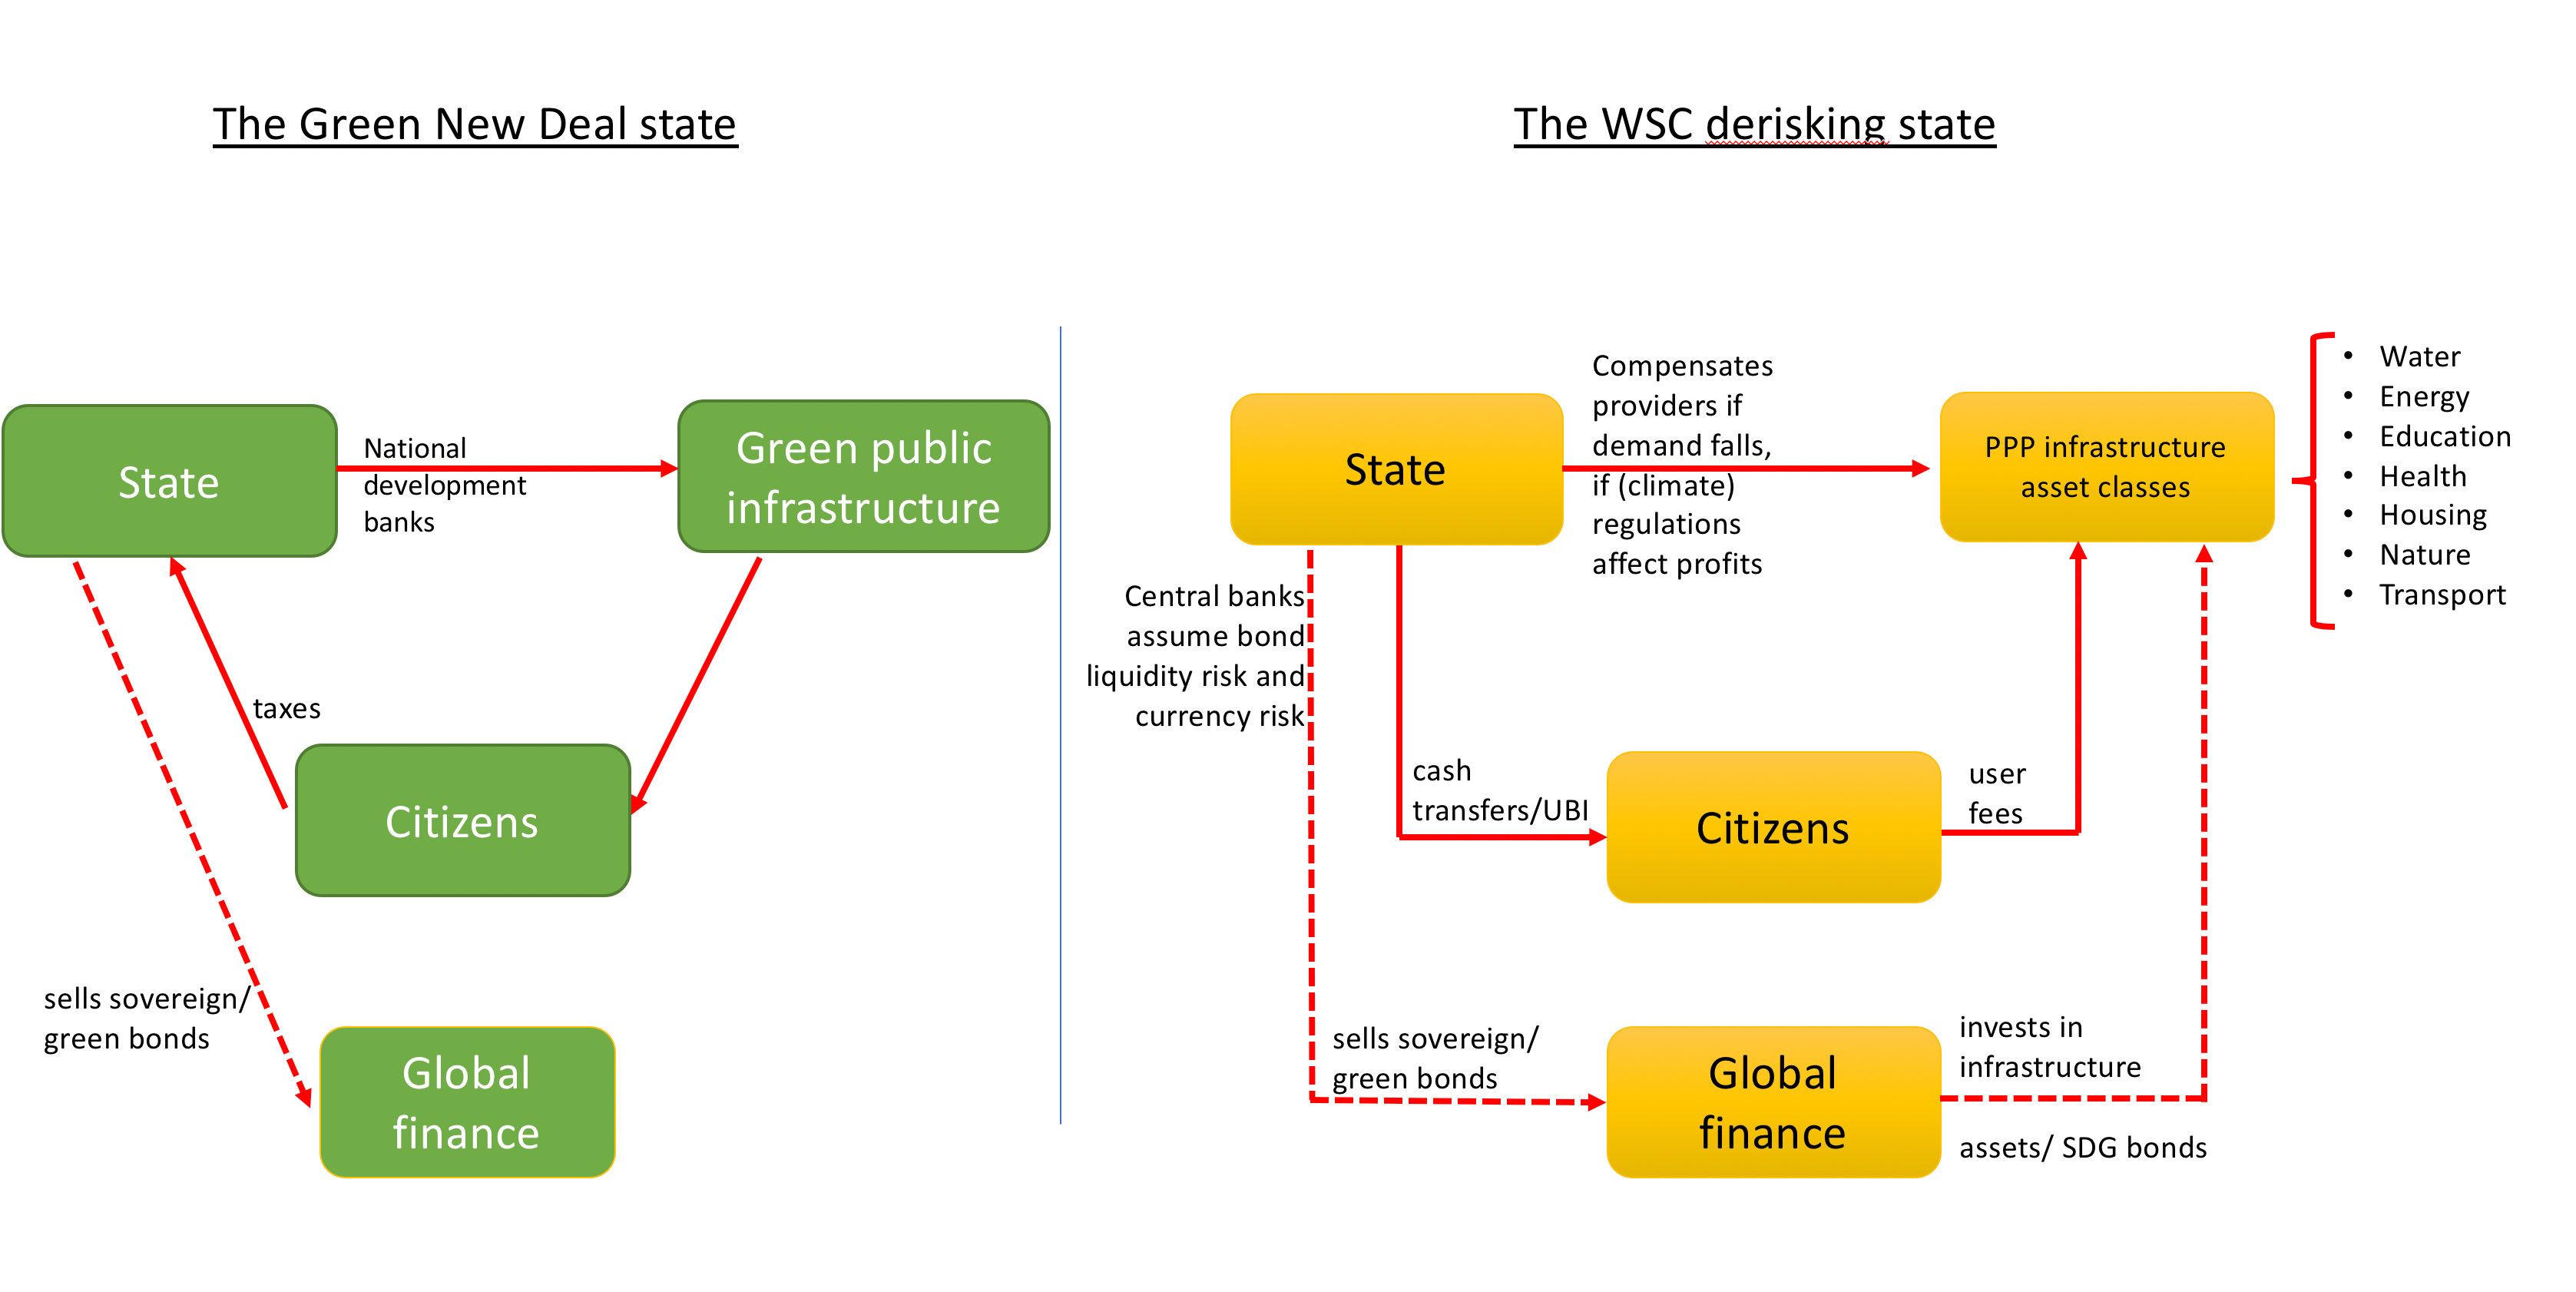
\includegraphics{fig/WSC_State.png}

In the derisking mode of governance, the state designs a menu of sector-specific policy
and financial derisking measures to encourage PPPs, accepts that this involves the
commodification of infrastructure via user-fees but puts in place cash
transfers/universal basic income schemes to mitigate the potential exclusion of the poor
from these services. That the derisking state does distributional politics through cash
transfers paradoxically accommodates calls for rethinking welfare politics as wage
labour becomes increasingly precarious.
Cash transfers enable the poor to access commodified public services,
and where these are not large enough, the state steps in to guarantee cash flows to investors.

Thus, development is not simply one-side defined by the political economy of capital,
but more specifically, by financial capital seeking to expand to new
areas, for which it colonises the infrastructure of the state. Financial capital no longer
just drags the poor into the embrace of the market, but also the state.

The derisking state can thus be understood as a project that seeks to extend the
infrastructural dependence of the state on finance -- and thus the infrastructural power
of the latter -- from its two traditional domains of monetary and fiscal policy to other
arenas of the government.

Derisking is not just about the transfers of risks to the state.
It is also about exercising infrastructural power to prevent
(regulatory) risks from materialising.

Derisking involves the central bank taking on its balance sheet bond liquidity and
currency market risks.

The legal battles to code capital into development asset
classes requires the state to take risks from the private sector onto its balance sheet, in
a clandestine reorienting of public resources that maintains the ideological commitment
to `fiscal responsibility'.

The WSC state assumes demand risk in user-fee based (social) infrastructure and
political risk that future governments might (re-)nationalize commodified
infrastructure or introduce tighter regulations, ranging from labour laws to climate
regulations that would affect profitability.

Uruguay's PPP law, passed by the
Mujica government in 2011, caps the total direct and contingent liabilities generated by
PPPs for the state to 7\% of the previous year's GDP, and fiscal transfers to private
operators to 0.5\% of previous year's GDP.

The fiscal costs of protecting investors from demand volatility will rise rapidly as
extreme climate events accelerate. Indeed, the climate crisis creates political and
demand risks that institutional investors need de-risking for.

The WSC protects investors against the political risks associated with green
developmental states. The green developmental state would prioritise the reorientation
of finance towards low-carbon activities. This requires a public taxonomy of green/dirty
assets that overcomes the shortcomings of private ESG ratings, and policies to penalize
dirty assets (through capital requirements or haircuts) 21 . Yet in the Wall Street
Consensus framework, such policies would classify as political risks, and require the
state to compensate their holders.

In its strategy to mutate climate risks into political and demand risks, private finance
may have found an important ally. Central banks conceptualize the immediate impact
of tighter climate rules regulation that increase the cost of funding or dramatically
change asset values as \emph{transition risks}.
The faster the low-carbon
transition, it is argued, the higher the potential that transition risks affect financial
stability, thus binding central banks in political trade-offs that privilege incremental
green regulatory regimes and accommodate greenwahing, however urgent the climate
crisis. Indeed, when central banks prioritize transition risks, they effectively rely on
private finance to drive the climate agenda, with their coordinating role focused on
subsidizing green assets, via so-called `green quantitative easing'.

In seeking to enlist central banks in the political coalitions against biting climate
regulation, the Wall Street Consensus constrains the green developmental states
directly, by making it liable for transition risks that can be framed as political and
demand risks, and indirectly, by reducing the public resources and central bank support
for Green New Deal programs that can effectively manage transition risks. The de-
risking state and the green developmental state can hardly co-exist, particularly within
market-based financial structures.

\textbf{Derisking market-based finance (formerly known as shadow banking)}

The turn to private finance as vehicle for sustainable development requires a change in
financial structures to accommodate the portfolio glut. It makes shadow banking,
understood as the production (via securitization) and financing (via wholesale funding
and derivative markets) of tradable securities, the desirable structure for financial
systems across the Global South. Indeed, the WSC consolidates
several global initiatives to restructure bank-based financial systems into market-based
finance or shadow banking,
where institutional investors can easily purchase local bonds (securities), including
infrastructure-backed securities, and finance as well as hedge their securities positions
via repos and derivative markets. Structural policies shift from developmental states'
concern with the productive structure, to the financial system.

The Financial Stability Board announced in 2015 that its new priority would be to transform
shadow banking into resilient market-based finance, which it defined as securities,
derivatives and repo markets.

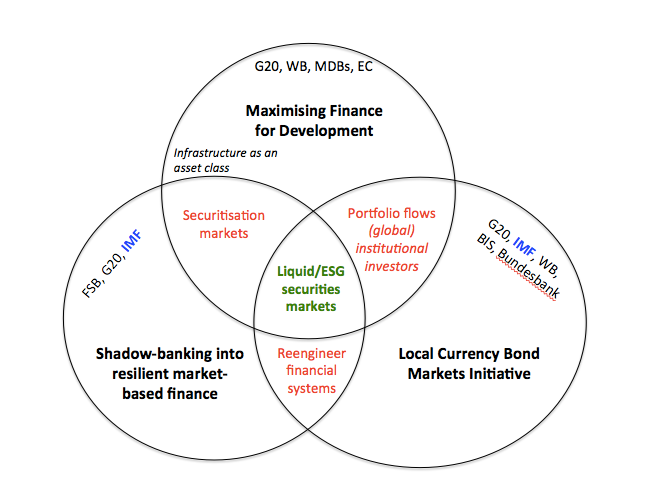
\includegraphics{fig/new_development_finance.png}

Figure: The turn to securities markets/market-based finance in international development

In sum, the organizational promoters of the Wall Street
Consensus championed in a multiplicity of global regulatory spaces the idea that
financial structure change is critical to attract the portfolio glut.

The
securitization of infrastructure loans would create both highly rated, low-return
tranches suitable for conservative pension funds/asset managers and lower-rated,
higher return tranches suitable for risk-driven investors. It would also accelerate lending
to infrastructure projects, constrained by Basel III rules for banks.

Since market-based finance is more systemically vulnerable than traditional bank-based
systems, the Wall Street Consensus assigns a triple de-risking role to central banks: in
bond markets and currency markets as market-makers of last resort,
and, forced by the inevitable consequences of green washing, as climate rescuers of last
resort, for assets left devalued by extreme climate events.
Some derisking
interventions, particularly in government bond markets, are at odds with the ideological
premises of central bank independence. Thus, the process of implicating central banks
in upholding the institutional basis of the derisking-centred accumulation regime is
incremental. It builds on crises such as the COVID19 pandemic to normalize new
derisking practices.

Greenwashing, like any
other regulatory arbitrage, eventually confronts its architects with the systemic
problems it feeds -- extreme climate events will devalue carbon-intensive assets and
greenwashed assets. The political logic of the Wall Street Consensus calls for central
banks to rescue the holders of last resort for carbon-intensive assets (Jahnke, 2019), to
risk-proof their portfolios, taking on its balance sheet the consequences of systemic
greenwashing.

`Development aid is dead, long-live private finance!'

\emph{Conclusion}

The Wall Street Consensus re-imagines international development interventions as
opportunities for global finance. In the new `development as derisking' paradigm,
institutional investors and asset managers are able to influence, if not altogether shape,
the terms on which poor countries join the global supply of `SDG' securities.
Multilateral development banks lead the efforts to design the ``de-risking''/subsidies
measures that seek to protect global investors from political risk or the demand risk
associated with privatized public services.

Equally important, this is a state-building project that puts in place the institutional
basis for a new regime of derisking as accumulation. The state comes under pressure
to institutionally codify risk-proofing arrangements, guaranteeing private financial
profits in the name of aligning sustainable projects with the preferred risk/return profile
of institutional investors. This includes adopting the US model of private pensions and
insurance to create local institutional investors. The tendency toward concentration in
the asset management sector (to exploit economies of scale and scope) may result in
Global North asset managers absorbing the funds of poor countries' institutional
investors and making allocative decisions on a global level.

In pushing for financial system change, development as derisking threatens to render
obsolete the old developmental banking model that put finance in the service of well-
designed industrial strategies. Development banks join the efforts of constructing and
derisking development asset classes. This is a political choice. Developmental banking
can arguably better serve a sustainability agenda because banks can easier include,
monitor and enforce safeguard policies in long-term relationships with customers. Most
countries with a successful experience of industrialisation relied on public development
banking as a critical pillar of industrial policies (Naqvi et al, 2018). Public development
banking allowed the developmental state to derisk via long-term loans to industrial
sectors identified as strategic by an industrial policy aimed at promoting the
international competitiveness of local firms.

This re-engineering of financial systems in the Global South, threatens the space for
alternative development strategies, and for a green developmental state. Government
capacity to design autonomous policies, in many poor countries severely eroded by
structural adjustment, will be further eroded by pressures to allocate scarce resources
to creating the conditions for private development finance.

\href{https://onlinelibrary.wiley.com/doi/abs/10.1111/dech.12645}{Daniela Gabor (2021) The Wall Street Consensus (Paywall)}
\href{pdf/Gabor_2021_Wall_Street_Consensus.pdf}{Draft (pdf)}

\hypertarget{imperialism-and-financialism}{%
\section{Imperialism and Financialism}\label{imperialism-and-financialism}}

\emph{Bichler \& Nitzan}

Over the past century, the nexus of imperialism and financialism has become a major axis
of Marxist theory and praxis. Many Marxists consider this nexus to be a cause of worldy
ills, but the historical role they ascribe to it has changed dramatically over time. The key
change concerns the nature and direction of surplus and liquidity flows. The first
incarnation of the nexus, articulated at the turn of the twentieth century, explained the
imperialist scramble for colonies to which finance capital could export its `excessive'
surplus. The next version posited a neo-imperial world of monopoly capitalism where the
core's surplus is absorbed domestically, sucked into a `black hole' of military spending
and financial intermediation. The third script postulated a World System where surplus is
imported from the dependent periphery into the financial core. And the most recent
edition explains the hollowing out of the U.S. core, a `red giant' that has already burned
much of its own productive fuel and is now trying to `financialize' the rest of the world in
order to use the system's external liquidity. This paper outlines this chameleon-like
transformation, assesses what is left of the nexus and asks whether it is worth keeping.

Our aim is to highlight the historical development of the
nexus of imperialism and financialism,
particularly the loose manner in which it has been altered --
to the point of meaning everything and nothing.

The paper comprises two parts. The first part examines the different schools. It
traces the transmutation of the nexus -- from its first articulation in the early twentieth
century, to the version developed by the Monopoly Capital school, to the arguments of
dependency and Word Systems analyses, to the thesis of hegemonic transition. The
second part offers an empirical exploration. Focusing specifically on the hegemonic
transition hypothesis, it identifies difficulties that arise when the theory meets the
evidence and assesses their significance for the century-old nexus.

\textbf{Empire and Finance}

The centralization of capital altered the political landscape. Instead of
the night-watchman government of the laissez-faire epoch, there emerged a strong, active
state.
The laissez-faire capitalists of the earlier era saw little reason to share their profits
with the state and therefore glorified the frugality of a small central administration and
minimal taxation. But the new state was no longer run by hands-off liberals. Instead, it was
dominated and manipulated by an aggressive oligarchy of `finance capital' -- a coalition of
large bankers, leading industrialists, war mongers and speculators who needed a strong
state that would crack down on domestic opposition and embark on foreign military
adventures.

The concentrated financialized economy, went the argument, requires pre-capitalist colonies
where surplus capital can be invested profitably; and the cabal of finance capital, now in
the political driver's seat, is able to push the state into an international imperialist
struggle to obtain those colonies.

At the time, this thesis was not only totally new and highly sophisticated; it also
fit closely with the unfolding of events. It gave an elegant explanation for the imperial
bellicosity of the late nineteenth century, and it neatly accounted for the circumstances
leading to the great imperial conflict of the first `World War'.

\textbf{Monopoly Capital}

In the brave new world of oligopolies, the emphasis on non-price competition
speeds up the pace of technical change and efficiency gains, making commodities cheaper
and cheaper to produce. But unlike in a competitive system, where market discipline
forces firms to pass on their lower costs to consumers, under the new circumstances, cost
reductions do not translate into falling prices. The prevalence of oligopolies creates a
built-in inflationary bias that, despite falling costs, makes prices move up and sometimes
sideways, but rarely if ever down.

This growing divergence between falling costs and rising prices increases the
income share of capitalists, and that increase reverses the underlying course of capitalism.
Marx believed that the combination of ever-growing mechanization and ruthless
competition creates a tendency of the rate of profit to fall. But the substitution of
monopoly capitalism for free competition inverts the trajectory. The new system
is ruled by an opposite `tendency of the surplus to rise'.

The early theorists of imperialism, although using a different vocabulary,
understood the gist of this transformation. And even though they did not provide a full
theory to explain it, they realized that the consequence of that transformation was to shift
the problem of capitalism from production to circulation (or in later Keynesian parlance,
from `aggregate supply' to `aggregate demand'). The new capitalism, they pointed out,
suffered not from insufficient surplus, but from too much surplus, and its key challenge
now was how to `offset' and `absorb' this ever-growing excess so that accumulation could
keep going instead of coming to a halt.

\textbf{Black Hole: The Role of Institutionalized Waste}

Until the early twentieth century, it seemed that the only way to offset the growing excess
was productive and external: the surplus of goods and capital had to be exported to and
productively invested in pre-capitalist colonies. But as it turned out, there was another
solution, one that the early theorists hadn't foreseen and that the analysts of Monopoly
Capital now emphasized. The surplus could also be disposed off unproductively and
internally: it could be wasted at home.

`Waste' denoted expenditures that are
necessary neither for producing the surplus nor for reproducing the population, and that
are, in that sense, totally unproductive and therefore wasteful. These expenditures absorb
existing surplus without creating any new surplus, and this double feature enables them to
mitigate without aggravating the tendency of the surplus to rise.

Use high military spending as a way to
secure the internal stability of U.S. capitalism.

The magnitude of military expenditures has no obvious ceiling: it
depends solely on the ability of the ruling class to justify the expenditures on the grounds
of national security. Similarly with the size of the financial sector: its magnitude expands
with the potentially limitless inflation of credit. This convenient expandability turns
military spending and financial intermediation into a giant `black hole'.

Spearheaded by U.S.-based multinationals and no longer hindered by inter-
capitalist wars, argued the theorists, the new order of monopoly capitalism has become
increasingly global and ever more integrated. And this global integration, they continued,
has come to depend on an international division of labour, free access to strategic raw
materials and political regimes that are ideologically open for business. However, these
conditions do not develop automatically and peacefully. They have to be actively
promoted and enforced.

Military spending comes to serve a dual role: together with the
financial sector and other forms of waste, it propels the accumulation of capital by black-
holing a large chunk of the economic surplus; and it helps secure a more sophisticated
and effective neo-imperial order that no longer needs colonial territories but is every bit
as expansionary, exploitative and violent as its crude imperial predecessor.

\textbf{Dependency}

The imperial powers relentlessly and systematically
undermined the socio-economic fabric of the periphery, making it totally dependent on
the core. And when decolonization finally started, the periphery found itself unable to
take off while the capitalist core prospered.
At that
point, there was no longer any need for core states to openly colonize and export capital
to the periphery. Using their disproportionate economic and state power, the former
imperialist countries were now able to hold the postcolonial periphery in a state of
debilitating economic monoculture, political submissiveness and cultural backwardness
-- and, wherever they could, to impose on it a system of unequal exchange.

This logic of dependent underdevelopment was first articulated during the
1950s and 1960s as an antidote to the liberal modernization thesis and its Rostowian
promise of an imminent takeoff.

Whereas earlier Marxist
theorists of imperialism accentuated the centrality of exploitation in production,
dependency and World-Systems analysts shifted the focus to trade and unequal
exchange. And while previous theories concentrated on the global class struggle,
dependency and World-Systems analyses spoke of a conflict between states and
geographical regions.

\textbf{Red Giant: An Empire Imploded}

`Financialization' is no longer a panacea for the
imperial power. On the contrary, it is a `sign of autumn', prime evidence of imperial
decline.

Finance (along with other
forms of waste) helps the imperial core absorb its rising surplus -- and in so doing
prevents stagnation and keeps accumulation going. But there is a price to pay. The
addiction to financial waste ends up consuming the very fuel that sustains the core's
imperial position: it hollows out the core's industrial sector, it undermines its productive
vitality, and, eventually, it limits its military capabilities. The financial sector itself
continues to expand absolutely and relatively, but this is the expansion of a `red giant' --
the final inflation of a star ready to implode.

The process leading to this implosion is emphasized by theories of hegemonic
transition.

The maturation of a hegemonic power -- be it Holland in the
seventeenth century, Britain in the nineteenth century or the United States presently --
coincides with the `over-accumulation' of capital.

This over-accumulation -- along with growing international rivalries,
challenges and conflicts -- triggers a system-wide financial expansion marked by soaring
capital flows, a rise in market speculation and a general inflation of debt and equity
values.
The financial expansion itself is led by the hegemonic state in an attempt to
arrest its own decline, but the reprieve it offers can only be temporary. Relying on finance
drains the core of its energy, causes productive investment to flow elsewhere and
eventually sets in motion the imminent process of hegemonic transition.

The United States benefited from being able to control,
manipulate and leverage this expansion for its own ends.
The growing severity of recent financial, economic and military crises suggests
that this ability has been greatly reduced and that U.S. hegemony is now coming to an end.

\textbf{End of Nexus?}

`Financialization' has not worked for the hegemonic power: despite the alleged
omnipotence of its Wall Street-Washington Complex, despite its control over key
international organizations, despite having imposed neoliberalism on the rest of the
world, and despite its seemingly limitless ability to borrow funds and suck in global
liquidity -- the bottom line is that the net profit share of U.S.-listed corporations has kept
falling and falling.

Of course, this isn't the first time that a monkey wrench has been thrown into the wheels
of the ever-changing nexus of imperialism and financialism. As we have seen, over the past
century the nexus has had to be repeatedly altered and transformed to match the
changing reality. Its first incarnation explained the imperialist scramble for colonies to
which finance capital could export its `excessive' surplus. The next version talked of a neo-
imperial world of monopoly capitalism where the core's surplus is absorbed domestically,
sucked into a `black hole' of military spending and financial intermediation. The third
script postulated a World System where surplus is imported from the dependent
periphery into the financial core. And the most recent edition explains the hollowing out
of the U.S. core, a `red giant' that has already burned much of its own productive fuel and
is now trying to `financialize' the rest of the world in order to use the system's external
liquidity.
Yet, here, too, the facts refuse to cooperate: contrary to the theory, they suggest
that the U.S. `Empire' has followed rather than led the global process of `financialization',
and that U.S. capitalists have consistently been less dependent on finance than their peers
elsewhere.

\href{http://bnarchives.yorku.ca/329/}{Bichler \& Nitzan (2012) Imperialism and Financialism}
\href{pdf/Bichler_Nitzan_2012_Imperialism_and_Financialism.pdf}{(pdf)}

\hypertarget{money-1}{%
\chapter{Money}\label{money-1}}

\begin{quote}
Money is the alienated essence of man's labour and life; and this alien essence dominates him as he worships it. (Karl Marx)
\end{quote}

\hypertarget{central-banks-1}{%
\chapter{Central Banks}\label{central-banks-1}}

In managing our economy with disembedded measures of wealth,
the world's central bankers are effectively agents of the sustainability crisis. They may not
wish to be unsustainable by personal inclination, but they certainly are by professional
obligation because of how they are duty-bound to act.
An entirely foreseeable response to the climate emergency is that people in wealthier
countries may choose to pare back their consumption of non-essentials. Certainly, not
everyone has the luxury to do this, but the obvious solution of ``buying less stuff'' has become
an articulated idea in wealthy countries. ``Flight shaming'' and ``consumption shaming'' are new
memes. Articles in multiple UK newspapers have challenged readers to see if they can go a
year without buying any new clothes, contravening the media's normal practice of generally
trying to coax the economy along. (It buoys the advertising revenue).
Such behaviours would amount to a direct hit on GDP in developed countries, where personal
consumption can represent two-thirds of the total. Critically, any such reduction in
consumption will likely show up as a deflationary decline in economic activity that the world's
central banks are on hair-trigger alert to prevent. The large and powerful financial
bureaucracy stands ready to provide immediate stimulus to any perceived flagging of
measured economic activity.
Hence, the arrangement most populations in the world currently live under is that should they
collectively choose to buy less, more money will be printed until they have changed their
mind. Effectively, our exhausted ecosystem is gasping for a lull in measured economic activity
that our financial authorities are pledged to never let happen.

\href{pdf/Austin_2021_Pigou_\%20and_the_dropped_stitch_of_economics_RWER95.pdf}{Duncan Austin: Pigou and the dropped stitch of economics RWER95 (pdf)}

\hypertarget{central-bank-independence-1}{%
\section{Central Bank Independence}\label{central-bank-independence-1}}

\hypertarget{market-neutrality}{%
\subsection{Market Neutrality}\label{market-neutrality}}

The principle of market neutrality posits that corporate bonds purchased under the ECB's €270bn corporate sector purchase programme should be made in a `neutral' way: they should reflect the overall eligible market to ensure they do not distort the relative pricing of securities. Given the concentration of carbon-intensive industries in the corporate bond universe, this has resulted in a carbon-biased portfolio. This is problematic as it exposes the ECB to climate-related risks. And yet central bankers have so far been reluctant to question market neutrality for fear of losing their independence.

\href{https://www.omfif.org/2021/02/ecb-market-neutrality-crumbling/}{Kyriakopoulou}

\emph{Klooster Abstract}

Monetary policy operations in corporate security markets confront central
banks with choices that are traditionally perceived to be the prerogative of
governments. This article investigates how central bankers legitimise
corporate security purchases through a comparative study of the
European Central Bank (ECB) and the Swiss National Bank (SNB). As we
show, central bankers downplay the novelty of corporate security
purchases by relying on familiar pre-crisis justifications of Central Bank
Independence. Citing an ideal of `market neutrality', central banks
present corporate security purchases as pursuing a narrow objective of
price stability and obfuscate their distributive consequences. In this way,
central bankers depoliticise corporate security purchases: they reduce
the potential for choice, collective agency, and deliberation concerning
both the pursuit of corporate security purchases and the choices made
in implementing these policies. We also describe the undesirable
democratic, social and environmental dimensions of these practices,
which we propose to address through enhanced democratic
accountability.

\emph{Klooster Memo}

The past decades saw central banks acquire considerable independence from democratic institutions
(McNamara 2002, Singleton 2010). Governments justified their decision to delegate monetary policy
by relying on a narrow conception of monetary policy. This conception focuses on the setting of short
term interest rates to achieve a long-term objective of stable price levels. A crucial element in the
justification of central bank independence is the idea that monetary policy is an apolitical, technical
area of policymaking (Marcussen 2009). The loss of democratic control that results from the creation
of an independent central bank was also thought to be minimal, because distributive choices would
remain with elected governments, who both decided on the central bank mandate and retained the
use of fiscal instruments to achieve their distributive objectives. In this way, governments depoliticised
monetary policy in the sense of reducing the potential for choice, collective agency, and deliberation
around the use of monetary policy

The Global Financial Crisis (GFC) led central bankers to move far beyond the narrow task assigned
to them under the traditional justification of Central Bank Independence (CBI)
To rescue a global financial system on the brink of collapse, central bankers assumed new roles as lenders and market makers of last resort.

Central bankers, meanwhile, are openly concerned that the use of unconventional tools threatens
their independence.
When independent regulatory agencies extend their power, political authorities often seek to regain
control.
Central bankers, accordingly, try to counteract repoliticisation and these efforts
shape their policies.

To investigate the simultaneously occurring processes of politicisation and depoliticisation
we investigate how central bankers relate to the political dimensions of their
new unconventional policies.

QE increases wealth inequalities.

Central bankers depoliticise their security purchases by subsuming
them under the pre-crisis justification of CBI.

Central bankers present themselves as pursuing price stability,
while in reality engaging in these purchases for reasons that are entirely unrelated to price stability.

\emph{`Market Neutrality'}

Rather than acknowledging and
managing the market impact of their policies, central bankers pursue `market neutrality', e.g.~they
seek to minimise the impact of their purchases on the relative prices of financial assets.

Central bankers keep decisions on new monetary instruments in the domain of their
expert judgment, and thereby outside the domain of democratic politics.

As a consequence of their effort to make corporate security purchases market neutral,
these programmes are insufficiently sensitive to environmental and societal concerns.

Depoliticisation of monetary policy: First, independent
central banks treat monetary policy as having a narrow objective, which can be achieved with a
clearly-defined toolbox and, second, central bankers treat distributive consequences as insignificant
and sanctioned by the central bank's mandate.

\href{https://www.tandfonline.com/doi/epub/10.1080/13563467.2019.1657077?needAccess=true}{Klooster (2021) The Myth of Market Neutrality}
\href{pdf/Klooster_2021_Myth_of_Market_Neutrality.pdf}{(pdf)}

The new exogenous money is exogenous transition shocks in the climate change debate.
Fortunately, Bank of England cannot hide behind that rock because of their new climate mandate.

Remember, Mark Carney's `tragedy of the horizons' speech identified two main risks of climate crisis:
- physical risks (climate events)
- transition risks - from green policies to accelerate transition to low-carbon

Now, central banks are confronted with an unpleasant conundrum that reveals the deeply political nature of their operations:
greening monetary policy (collateral, unconventional bond purchases) means endogenous transition risks

So, in a have your cake and eat it moment, there is a growing tendency in central bank communities to pretend that all transition risks come from the fiscal side (carbon pricing)

It wouldn't be surprising to find the exogenous transition shocks approach in the ECB's monetary policy strategy review, despite \citet{Lagarde}
and other's recognition that central banks cannot longer hide behind the `market neutrality' argument.

\href{https://twitter.com/DanielaGabor/status/1384837864412917765}{Gabor (Twitter)}

\hypertarget{financial-stability-1}{%
\section{Financial Stability}\label{financial-stability-1}}

\hypertarget{climate-risk-1}{%
\subsection{Climate Risk}\label{climate-risk-1}}

\textbf{BIS Recommendations}

This report provides an overview of conceptual issues related to climate-related financial risk
measurement and methodologies, as well as practical implementation by banks and supervisors.

The report contains five key findings:
First, climate-related financial risks have unique features, necessitating granular and
forward-looking measurement methodologies.

Second, to date, measurement of climate-related financial risks by banks and supervisors
has centred on mapping near-term transition risk drivers into counterparty and portfolio exposures.

Third, banks and supervisors have predominantly focused on assessing credit risk, as they
advance in applying methods to translate climate-related exposures into categories of financial risk.

Fourth, while banks and supervisors remain at an early stage of translating climate-related
risks into robustly quantifiable financial risk, work continues to gather pace

Fifth, key areas for future analytical exploration relate to measurement gaps in data and
risk classification methods, as well as methodologies suitable for assessing long-term climate
phenomena not always of a standard nature.

\href{https://www.bis.org/bcbs/publ/d518.htm}{BIS (2021) Climate Risk}
\href{pdf/BIS_2021_Climate_Risk.pdf}{(pdf)}

\textbf{Institutional Dynamics}

\emph{Baer Abstract}

This article studies how institutional dynamics might affect the implementation of climate-
related financial policies. First, we propose a three-dimensional framework to distinguish: i)
motives for policy implementation (prudential or promotional); ii) policy instruments
(informational, incentive or coercive); and iii) implementing authorities (political or
delegated). Second, we use this framework to show how sustainable financial interventions in
certain jurisdictions - most notably, Europe - rely solely on informational policies to achieve
both promotional and prudential objectives. Policymakers in other jurisdictions - e.g., China -
also implement incentive or coercive financial policies to achieve promotional objectives.
Third, we identify two main institutional explanations for this European `promotional gap': i)
limited control of political authorities on financial dynamics; and ii) strong powers and
independence of delegated authorities. This governance configuration leads to an institutional
deadlock in which only measures fitting with both political and delegated authorities'
objectives can be implemented. Finally, we discuss the scenarios that might originate from the
current institutional setting. We identify three possible evolutionary paths: i) a drift towards a
green financial technocracy; ii) a re-politicization of delegated authorities; iii) a move towards
fiscal-monetary coordination.

\emph{Baer Memo}

In 2017, the EU Commissioner Valdis Dombrovskis expressed his support to the idea of
introducing a `green supporting factor' in bank capital requirements to incentivize lending to
sustainable activities (Dombrovskis, 2017). The following year, the European Commission
included the idea of `incorporating sustainability in prudential requirements' in its sustainable
finance action plan (EC, 2018). This position was generally greeted with skepticism by most
central bankers and financial supervisors (see, among others: Dankert et al., 2018; Elderson,
2018; Rehn, 2018). It was emphasized that the aim of prudential rules is to mitigate financial
risk, not to steer private credit in any particular direction. \emph{According to central bankers and
financial supervisors, capital requirements should not discriminate between green and dirty
financial assets, unless clear evidence of risk differentials is available.}

This recent clash between public institutions raises deeper questions. For what purposes should
banking and financial regulation be used? And who should decide what the admissible
purposes are?

EU Banking regulation cannot be employed as a
policy tool to actively reallocate private financial resources towards sustainable investments.

In several emerging economies banking and financial regulation is instead
actively used to promote specific productive sectors.
Financial risk is still monitored, but stronger
weight is given to development (e.g., green) objectives.

The current status quo is unsustainable due to environmental constraints. At some
point, someone will need to introduce stronger promotional policies to steer credit towards
sustainable sectors. Given the distribution of responsibilities, missions, and powers crystallized
within the current institutional framework, these promotional efforts should be led by the
political authorities, leaving delegated authorities with a supporting role.

\href{pdf/Baer_2021_Institutional_Climate_Policy_Dynamics.pdf}{Baer (2021) Climate-related financial policies (pdf)}

\hypertarget{index-providers-1}{%
\chapter{Index Providers}\label{index-providers-1}}

\emph{Fitchner}

A silent revolution is happening in investing. It is a paradigm shift that will have a profound impact on corporations, countries and pressing issues like climate change.
A silent revolution is happening in investing. It is a paradigm shift that will have a profound impact on corporations, countries and pressing issues like climate change.
In 2019 there was a watershed in the history of finance. In the United States, the total value of actively managed funds was surpassed by passive funds. Globally, passive funds crossed US\$10 trillion (£7.7 trillion), a five-fold increase from US\$2 trillion in 2007.

This seemingly unstoppable ascent has two main consequences.

First, corporate ownership has become concentrated in the hands of the ``big three'' passive asset managers: BlackRock, Vanguard and State Street. They are already the largest owners of corporate America.

The second consequence relates to the companies that provide the indices that these passive funds follow. When investors buy index funds, they effectively delegate their investment decisions to these providers. Three dominant providers have become increasingly powerful: MSCI, FTSE Russell and S\&P Dow Jones Indices.

A silent revolution is happening in investing. It is a paradigm shift that will have a profound impact on corporations, countries and pressing issues like climate change. Yet most people are not even aware of it.

In a traditional investment fund, the decisions about where to invest the capital of the investors are taken by fund managers. They decide whether to buy shares in firms like Saudi Aramco or Exxon. They decide whether to invest in environmentally harmful businesses like coal.

Yet there has been a steady shift away from these actively managed funds towards passive or index funds. Instead of depending on a fund manager, passive funds simply track indices -- for example, an S\&P 500 tracker fund would buy shares in every company in the S\&P 500 in order to mirror its overall performance. One of the great attractions of such funds is that their fees are dramatically lower than the alternative.

In 2019 there was a watershed in the history of finance. In the United States, the total value of actively managed funds was surpassed by passive funds. Globally, passive funds crossed US\$10 trillion (£7.7 trillion), a five-fold increase from US\$2 trillion in 2007.
¿Le gusta lo que lee? ¿Quiere más?

This seemingly unstoppable ascent has two main consequences. First, corporate ownership has become concentrated in the hands of the ``big three'' passive asset managers: BlackRock, Vanguard and State Street. They are already the largest owners of corporate America.

The second consequence relates to the companies that provide the indices that these passive funds follow. When investors buy index funds, they effectively delegate their investment decisions to these providers. Three dominant providers have become increasingly powerful: MSCI, FTSE Russell and S\&P Dow Jones Indices.

With trillions of dollars migrating to passive funds, the role of index providers has been transformed.

In the past, index providers only supplied information to financial markets. In our new age of passive investing, they are becoming \emph{market authorities}.
Deciding who appears in the indices is not just something technical or objective. It involves some discretion by the providers and benefits some actors over others. By determining which players are included on the list, setting the criteria becomes an inherently political activity.

The three dominant index providers' income mainly derives from the funds replicating their indices, since they have to pay royalties for the privilege.
MSCI, FTSE Russell and S\&P Dow Jones will increase their role as \emph{a new kind of de facto
global regulators}.

This tightly interlinked group of three giant passive fund managers and three major index providers will largely determine how corporations tackle climate change. The world is paying little attention to the judgements they make, and yet these judgements look highly questionable. If the world is truly to get to grips with the global climate crisis, this constellation needs to be far more closely scrutinised by regulators, researchers and the general public.

\href{https://theconversation.com/three-financial-firms-could-change-the-direction-of-the-climate-crisis-and-few-people-have-any-idea-131869}{Fitchner in The Conversation}

\emph{Petry}

Since the global financial crisis, there is a massive shift of assets towards index
funds. Rather than picking stocks, index funds replicate stock indices such as the
S\&P 500. But where do these indices actually come from? This paper analyzes the
politico-economic role of index providers, a small group of highly profitable firms
including MSCI, S\&P DJI, and FTSE Russell, and develops a research agenda from an
IPE perspective. We argue that these index providers have become actors that exer-
cise growing private authority as they steer investments through the indices they
create and maintain. While technical expertise is a precondition, their brand is the
primary source of index provider authority, which is entrenched through network
externalities. Rather than a purely technical exercise, constructing indices is inher-
ently political. Which companies or countries are included into an index or excluded
(i.e.~receive investment in- or outflows) is based on criteria defined by index pro-
viders, thereby setting standards for corporate governance and investor access.
Hence, in this new age of passive asset management index providers are becoming
gatekeepers that exert de facto regulatory power and thus may have important
effects on corporate governance and the economic policies of countries.

Index mutual funds have been available since the late 1970s and the first ETFs
have been launched in the early 1990s. However, investors shunned them for a long
time. But after the global financial crisis growth of index funds has accelerated mas-
sively.

An unprecedented
money mass-migration from active to passive funds, which is rational as most
actively managed funds are unable to beat broad market indices over longer time
periods but charge high fees.

One crucial, yet largely unstudied element of this new era is that
index funds effectively delegate their investment decisions to index providers. Index
providers are the firms that create and maintain the indices on which passive funds
rely and to which asset managers have to pay fees if they use them.

Similar to passive asset management, which is dominated by the `Big Three' of
BlackRock, Vanguard, and State Street (Fichtner et al., 2017), the global index pro-
vider industry is very concentrated. Just three firms, MSCI, S\&P Dow Jones Indices
(DJI) and FTSE Russell, hold a combined market share of almost 80\%.

While global index revenues totaled a record US\$2.7 billion in 2017,
their profit margins that stand out as exceptionally high.
MSCI reports an operating margin of over 60\% for its index segment in 2018.
Index providers operate in an oligopolistic industry,
which has high barriers to competition.

During the last decade the big index providers have had
much higher growth than most other financial companies, especially banks.

Index providers today occupy a position of growing
private authority, with decision-making and standard-setting capabilities that are
consequential in the global political economy. In the past, their indices primarily
served informational purposes. An index such as the S\&P 500 or the Nikkei was
primarily a numerical representation of a particular stock market. Indices served as
benchmarks against which analysts could gauge the performance of stocks. While
the decisions of index providers had some impact on actively managed funds, the
rise of passive investing transformed their role in a significant way. Today, they de
facto steer capital with their indices as inclusions of firms or countries to an
index can lead to inflows of billions of US\$ while exclusions can cause large quasi-
automatic outflows. Constructing indices is therefore not a purely technical exer-
cise. Index providers have significant discretion in devising their methodologies.

The methodology of the pivotal S\&P 500
index was changed at least eight times between 2015 and 2018. Underlying their
seemingly technical exercise are decisional discretion and normative assumptions
about `good' corporate governance and `free' markets. Index providers therefore
play a role as standard-setters: their notions on what constitutes good corporate
governance at the level of the firm and a favorable investment environment at the
level of (national) markets helps or hinders firms and countries in attracting cap-
ital, essentially deciding what is investment-worthy in global financial markets.
This combination of standard-setting and legitimate decision-making power means
that index providers have gained a position of private authority in capital markets
with profound politico-economic consequences.
Today index providers have become important counterparts for states.

Index providers increasingly are
to equity markets what credit rating agencies are to bond markets, crucial
`coordination service firms' that exercise private authority and effectively
set standards for the behavior of other firms and even countries

Their new authority was not delegated from
the public sphere, but gradually emerged as part of a transformation of the index
provider industry -- from primarily supplying information about markets to
becoming private authorities that are able to set standards on corporate governance and
steer international capital flows.

Take for example FTSE Russell, S\&P DJI and
MSCI's emerging market indices; the index providers' recent decision to include
countries such as China and Saudi Arabia to their indices is expected to result in a
`seismic shift' of over US\$120 billion in active and passive fund flows by 2020.

Indices act as `prisms' through which fund managers view the investible world.

Financial market indices are far from objective.

They represent `deliberate decisions'
made by index providers as every index is a managed portfolio whose composition
is decided by the respective index provider.

While these
simplified numerical representations might seem objective and technical, they are
actually based on complex and (often contested) normative values. Moreover, proc-
esses of index production are inherently subjective activities.

Standard-setting is always political.

\emph{Distance Governance}

Indices and indicators have a governing effect on those that are being evaluated,
incentivizing the individuals, companies or states that are being assessed
to comply with the norms underlying those numerical representations,
as better performance has positive ideational and material effects,
enabling a form of `governance from a distance'

Critical gatekeepers that exert de facto regulatory power.

The emergence of private authority through the retreat of the state,
which provided a space for private actors such as firms to exercise authority.

Questions such as the public regulation of index providers.

Private authority is inherently relational, produced and
reproduced through ongoing interactions between the authority and non-authorities,
where the formers' decisions are considered as legitimate by the latter

Rather than coercion or self-interest, legitimacy is a `normative belief
by an actor that a rule or institution ought to be obeyed' and is based on how the
authority is `perceived' by non-authoritarian actorsRather than coercion or self-interest,
legitimacy is a `normative belief by an actor that a rule or institution ought to be obeyed'
and is based on how the authority is `perceived' by non-authoritarian actors.

Three conditions for index provider authority.
First of all, technical expertise to construct an index is a necessary -- but not sufficient.
Second condition; crucial for index provider authority is their brand recognition,
or more specifically the trust that the international investment community puts in their brands.
`Authority is socially constructed' and is ultimately based on
trust, which in turn is based on reputation.
The big three index providers are `brand managers'
: `at the end of the day, those products are homogeneous and exchangeable.
It's like water, there are small differences why Evian is more expensive {[} \ldots{} {]}.
Those are minimal differences, but the price tags are very different!
A third condition that underpins index provider authority lies in a set of net-
work externalities that reinforce the authority of the major index providers. As first
movers they have in effect `captured' different national (e.g.~S\&P 500 or FTSE 100)
and regional (Euro Stoxx 50) market segments with their indices.
These network externalities entrench the authority
that leading index providers derive from their brands. With these three conditions in
place, index providers have become private authorities in financial markets.

The authority of rating agencies developed within and was enabled by changing socio-
economic structures, i.e.~the growth of capital markets and the decline of banks as
allocators of credit, which created a demand for rating agencies' services for the
functioning of the then disintermediated structure of finance.

Authority is best understood as an effect of these circumstances, rather than as an entity or a
characteristic of an actor or institution' and `its existence is therefore not func-
tional, {[} \ldots{} {]} but always contingent on time, place, and circumstance.

Indices had at least some influence on asset managers as an
deviation from the relevant index could be conceived as a kind of risk management
metric.
However, indices only loosely anchored the asset allocation as most fund
managers had the discretion to choose both the degree of replicating the index as
well as the time period for doing so.

Changed fundamentally with the rise of passive investing in the mid-2000s.
Index providers began to influence capital flows in an immediate and comprehensive way.
Being a central
component of the index funds ecosystem conferred them -- gradually and only as a
side-effect of their business model -- a position of growing private authority in
financial markets.

The money mass-migration
towards passive investments, which significantly increased the nascent authority
of index providers as evermore funds directly tracked their indices. Whereas in
the past indices only loosely anchored fund holdings around a baseline, now they
had an instant, `mechanic' effect on the holdings of passive funds, `steering' cap-
ital flows. Increasingly, investments were not actively managed by fund managers
but passively invested into index mutual funds and ETFs

This makes sense as the vast
majority of actively managed funds have not been able to beat benchmark indices
over longer periods of time, while charging substantially higher fees than index
funds.

In order to track the performance of `the market', passively
managed funds replicate stock market indices such as the S\&P 500 or the MSCI
World. Rather than trying to generate `alpha' and outperform the market by pick-
ing stocks, these passively managed funds aim to generate `beta', simply replicat-
ing the performance of specific stock markets while minimizing fees.

By investing in an index, passive investors delegate decision-making about
where to invest to index providers. Index investing thus represents a form of
`delegated management' and every discretionary decision by index providers has a
`flow through effect on the investor's portfolio'

A substantial proportion of equity funds that officially are actively managed
funds (and therefore charge higher fees than index funds) but actually do not devi-
ate much from their benchmark indices. This is referred to as `closet indexing' or
`index hugging', and it is estimated that in the EU between 5-15\% of all equity
funds could fall into this category (ESMA, 2016). Therefore, the rise of passive
management also increases the authority of index providers vis- a-vis active man-
agement because by steering evermore passive capital index decisions now mechan-
ically move ever larger parts of the markets, creating a `pull effect' that actively
managed funds need to follow

Hedge funds and sovereign wealth funds (SWFs) generally have low degrees of rep-
licating indices (one exception is the Norwegian SWF, which almost invests like a
global ESG 5 index fund) and are fully discretionary to follow any index modifica-
tion.

Indices no longer merely measure markets. They move them.

Far from simply
providing information on `the market', index providers now offer a variety of cus-
tomized branded products, by either tweaking existing benchmarks or repackaging
proprietary trading strategies into indices which enable the functioning of (passive)
asset management capitalism.

The relationship between index providers and asset managers is intriguing. On
the one hand, asset managers depend on the large index providers to create their
products that are attractive to investors. On the other hand, they have an interest
to reduce the fees they have to pay for using indices. In theory, there are two ways
for competition to emerge in the index industry: through new index providers and
through self-indexing by asset managers. However, both have so far not been able
to break the oligopolistic market structure.

It is further difficult for challenger indices to gain benchmark status as network
externalities entrench the authority of the big index providers.

Index providers not only decide to include particular firms, they
also make decisions on in- and exclusions of entire markets, steering capital with
important politico-economic implications for states.

While many indices are strictly rule-based and thus only influence companies indirectly,
some indices -- including the S\&P 500, the world's most-tracked index -- have com-
mittees that make discretionary, less rule-based decisions.
While the majority of inclusions is rather mechanical
and influence is indirect, it is not uncommon that index decisions target individual
firms to set a `precedence' on a particular issue that then gets incorporated into
existing methodologies.

It has become standard practice for the majority
of key global stock indices to use only the market capitalization of firms for calcu-
lating the weight of companies. Market capitalization primarily derives from the
(future) profits of corporations. Even though that has changed somewhat in the
last decades, profit maximization is still not the exclusive goal of corporations from
countries such as France, Germany and Japan.

\emph{`reluctant regulators'}

`We're not activists. We're setting the minimum standards
that investors generally will accept, and our role is to build consensus amongst that
investor community as to what that minimum standard should be'.

The three big index providers are therefore best
seen as consensus-building agents that aggregate their own interests with those of
asset managers from developed economies, i.e.~mainly from Anglo-
American countries.

Index providers have become de facto private standard-setters over corporate governance.

By reclassifying individual countries, index providers effectively redraw the borders of
markets. Index providers set out the criteria that decide which countries are
`investment-worthy'.

Index providers decide whether to include countries
into their indices and whether to classify them as `frontier', `emerging' or
`developed' markets. 8 By additionally putting countries on watchlists for such inclu-
sions, exclusions or reclassifications, index providers create incentives for states to
comply with their rules.

MSCI in effect controls the definition of which countries
are ``emerging markets.
Criteria are set out in MSCI's Market Classification Framework, com-
prising three elements: economic development; size and liquidity; and investor
access. Economic development is not crucial as a criterion, neither are the size and
liquidity requirements (only 2-5 companies need to meet minimum requirements).
Investor access is the dealmaker/breaker for country classifications, and it is on this
that most indexing decisions are based

While index
decisions about company inclusions are often more indirect and not targeted at indi-
vidual companies, in the case of country reclassifications index providers take a much
more proactive role. As the following cases demonstrate, these deci-
sions have enormous consequences for states and their national stock markets.

MSCI has a quasi-regulatory function -- `even though MSCI is not a regulator, companies need
to abide, to respect their rules'.

\href{https://www.tandfonline.com/doi/full/10.1080/09692290.2019.1699147}{Petry (2021) Steering Capital}
\href{pdf/Petry_2021_Steering_Capital.pdf}{(pdf)}

\hypertarget{hedge-funds-1}{%
\chapter{Hedge Funds}\label{hedge-funds-1}}

In the midst of a global crisis, the hedge fund has prospered. The top fifteen hedge-fund managers earned an estimated \$23.2 billion last year, according to Bloomberg. Chase Coleman, the forty-five-year-old founder of Tiger Global Management, led the way, hauling in more than three billion for himself. The Financial Times took a more democratic view of the phenomenon, noting that the top twenty ``best-performing hedge fund managers of all time'' had provided more than sixty-three billion dollars for their investors during the coronavirus-driven market turmoil, ``making it the industry's best year of gains in a decade.''

Given the supremacy of hedge funds, it was both satisfying and terrifying to observe the recent boom and bust in the value of GameStop, a run driven by small-time speculators. Several hedge funds lost extraordinary amounts of cash---as in billions and billions of dollars---on financial derivatives.

Those who work at hedge funds are diligent about keeping who they are and what they do obscured behind a wall. Secrecy is intrinsic to the job description---for a hedge is a wall.

\href{https://www.newyorker.com/culture/culture-desk/a-brief-history-of-the-hedge-fund}{Kaufman in New Yorker: History of Hedge}

\hypertarget{institutional-investors-1}{%
\chapter{Institutional Investors}\label{institutional-investors-1}}

\hypertarget{esg-2.0-1}{%
\section{ESG 2.0}\label{esg-2.0-1}}

\emph{Segal}

\textbf{How Institutional Investors Encourage Corporations Bad Behavior}

Wittingly or unwittingly, pensions and endowments' investment strategies aid and abet activities that make the financial system more fragile.

The growing scale of institutions and the large amounts of money they need to deploy into high-risk investments is leading to consolidation among asset managers, higher global debt levels, short-term corporate behavior, and market instability.

Institutions' investment strategies are in conflict with environmental, social, and governance goals to which they are increasingly committing.

Pension funds, insurance companies, sovereign wealth funds and others need to deploy large amounts of capital efficiently because they themselves are so big.

Institutions' only option in many cases is to put billions of dollars to work in the largest public and private companies, Rothenberg explained. That results in companies, for example, taking on unsustainable amounts of debt.

There are incentives to layer on debt, much of which is supplied by capital markets and the shadow banking sector.

Ironically, institutional investors want to integrate ESG into their process, but they also contribute to corporate consolidation and huge debt burdens. Institutional investors are essentially contributing to some of their own problems in the way they allocate capital to leveraged loans, high-yield loans, collateralized loan obligations
and other higher risk products.

All of this adds to global systemic risks.
Unchecked increases in corporate debt result in increased systematic market risk that boomerangs back to investors and their portfolios
Existing approaches like Modern Portfolio Theory and ESG or impact investing frameworks don't focus on these potentially negative effects.

Perversely, as major central banks globally respond to the current crisis with rock bottom interest rates and new rounds of quantitative easing (QE), investors and companies are further incentivized to increase their exposure to high-risk debt and inflated asset valuations --- a situation that leaves society and markets vulnerable to a rise in interest rates or other unplanned challenges

\href{https://www.institutionalinvestor.com/article/b1r9js87jhyn8s/How-Institutional-Investors-Encourage-Corporations-Bad-Behavior}{Segal - Comment - Instititional Investor}

\emph{Rothenburg}

Many of our existing ESG and impact investing frameworks focus on issues at the
portfolio company level, but they do not take into account potential negative
impacts from capital structures and investors' influence in shaping them.
Asset allocation strategies can be in conflict with ESG objectives.

The conflict materializes in various interconnected ways, particularly from
institutional investors' role in increasing global debt levels and
fund manager and corporate consolidation.

For long-term, diversified institutional investors, or ``Universal Owners''
of the market, these dynamics eventually translate into lower financial returns.
For workers and communities, these dynamics translate into
greater precarity and inequality.

Potential solutions focus on diversifying asset allocation to
more regenerative investment structures and asset classes, building an
enabling environment through adjustments to team incentive structures, performance reviews,
benchmarking and valuation methodologies, and field-building.

Over the past decades, institutional investors have migrated up
the risk-return spectrum to asset classes with higher yields.
Investor allocations to private equity (PE), venture capital (VC), private debt (PD),
high yield bonds (HYBs), leveraged loans (LLs), and
collateralized loan obligations (CLOs), for instance,
have been growing steadily in response to a number of trends.
\emph{While such shifts in asset allocation may suit near-term goals,
such as meeting actuarial targets, this institutional allocation to higher risk asset
classes has also meant increased global debt burdens, corporate and
fund manager consolidation, and risk across capital structures,
resulting in fragility for companies, the real economy, and the stability of
financial markets.
The resulting risks are therefore shared not only by investors,
but also governments,workers, and communities alike.}

To optimize leverage ratios, companies may prioritize debt servicing or distributions to investors at the
expense of worker payrolls and benefits. Infrastructure and social infrastructure investments --- such as
power, water, roads, hospitals, nursing homes, housing, and cybersecurity --- might be structured in
such a way that provides access to end-users at unaffordable prices, or of poor quality, in order to meet
investor return expectations and therefore attract capital. Weak capital structures increase the risk of
restructurings or bankruptcies that are detrimental for stakeholders, such as workers. Stakeholders have
increasingly raised concerns about high leverage, coined ``financial engineering,'' particularly in the PE
asset class, for such reasons. 5 Yet studies produced over the past decades, inspired by PE, praise the
discipline of debt, and due to a number of additional factors, high leverage ratios are no longer confined
to the PE asset class and are prolific across public equity markets, as well.

In practice, the negative impacts of weak capital structures are typically being addressed piecemeal
through company-by-company interventions that focus on corporate operations, like a game of whack-
a-mole; but key roots of the problem --- the investment structures themselves --- are left unaddressed.

The unintended negative consequences of highly levered investments have been underexplored when it
comes to ESG and impact investing frameworks and practice. Matters relating to investment structures,
capital structures, leverage ratios, earnings calculations, valuation methodologies, benchmarking
approaches, and resulting asset allocation and portfolio construction are not typically within the realm
of ESG-related responsibilities.

Too much leverage is dangerous for all stakeholders.
While leverage looks like a neutral, bilateral accelerant, it
actually reduces financial resiliency at the very times when it might be most needed.

Systemic inequality has been shown to result in economic decline.

Neither Modern Portfolio Theory (MPT) nor ESG or impact investing frameworks
currently include a focus on potential negative impacts stemming from
investment structures.

Corporate debt burdens and leverage ratios are historically high, covenants are light, and
defaults and bankruptcies are being held at bay by government support
(e.g.~through fiscal and monetary policy) -- which is also funded by debt,
though at the sovereign level.

Corporate funding dynamics have changed since the Global Financial Crisis
(GFC), when banks came under heavy regulation that caused them to
restrict lending to smaller clients.
Capital markets, or the Non-bank Financial Intermediary
(``NBFI'' or ``Shadow Banking'') sector, has stepped in to fill this void.

The financial assets of the NBFI sector amounted to \$200.2 trillion in 2019,
accounting for nearly half of the global financial system in 2019, up from 42\%
in 2008

\emph{How Did We Get Here?}

For the past two decades, institutional asset owners have significantly shifted their overall asset
allocation strategy. Private markets -- including PE, PD, VC, infrastructure, and real estate - as well as LLs,
CLOs, and HYBs, have become much larger percentages of overall portfolios. There are a number of
reasons for these changes, including, but not limited to, ongoing declines in interest rates by major
global central banks, dynamics related to funding ratios of institutional investors such as pension funds,
growing interest in the illiquidity premium of private markets, benchmarking practices, investor
dissatisfaction with public markets, and increased opportunity for NBFIs to provide financing following
banking regulations resulting from the GFC. 16 Private capital assets under management (AUM) in 2019
was approximately US\$6.5 trillion, an increase of over US\$4 trillion over the past ten years.

\emph{Private Equity (PE)}

Investor demand is now so high for PE that many are concerned that the asset class is becoming crowded with capital.

Consolidated capital flows stems from the institutionalization of capital.
Markets have evolved from being dominated by individual investors to
having a large presence of institutional investors.
Institutional investors now hold over 40 percent of
global market capitalization of listed companies.

Institutional investors have sizable portfolios and must invest billions
if not trillions of dollars.
With such large chunks of capital to put to work,
they often find it challenging to invest in smaller fund managers,
smaller companies, and niche investment strategies due to a number of factors,
such as transaction costs.

Even when small deals perform well, which data suggests that they often do,
they are hard to justify because they do not meaningfully move the needle
in terms of overall portfolio returns.

A well-documented negative impact of consolidated capital flows to larger
fund managers is that
smaller, emerging, and innovative fund managers can be starved of capital.

\emph{Institutionalization of Capital}

The consolidation of capital among institutional investors is a double-edged sword. On the one hand,
institutions offer individual investors professional money management with multi-disciplinary staff and
robust internal infrastructure capable of constructing well-diversified portfolios. Size and scale can also allow
large allocators to influence corporate governance of portfolio companies, as well as negotiate more
attractive terms with fund managers. It is arguable that fees overall are reduced through these dynamics, and
strong ESG practices can be better advocated for. On the other hand, since large institutions need to put
significant amounts of capital to work, they often allocate to the largest managers and companies, thereby
resulting in consolidation of power, profit, influence, and opportunity among a shrinking pool of asset
managers and companies. 53 In order for large institutional investors to act as responsible Universal Owners
and effectively manage systematic risk, it will be critical for them to evaluate their asset allocation practices
for unintended negative consequences that not only impact the real economy, but also markets and their
long-term portfolios.

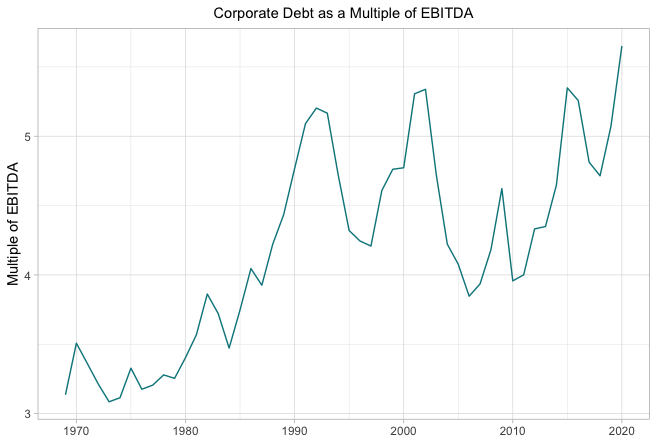
\includegraphics{fig/corporate_debt_ebitda.png}

This high-risk debt is not limited to private companies. A recent Forbes article highlights how, ``some of
the biggest firms in the United States\ldots{} have binged on low interest debt. Most of them borrowed more
than they needed, often returning it to shareholders in the form of buybacks and dividends. They also
went on acquisition sprees.''

From the corporate perspective, historically cheap credit due to low interest rates is attractive,
particularly when combined with the current tax deductibility of interest expense, studies suggesting
that highly leveraged capital structures do not negatively impact stock prices, and arguments that debt
adds discipline to corporate management. Yet debt and common uses of funds can increase risk for
other stakeholders. M\&A has been shown to contribute to corporate consolidation which can stifle
SMEs, innovation, suppliers, the quality and affordability of goods and services, labor's bargaining
power, and diversification for institutional investors. There is significant literature that explores
negative impacts of share buybacks in public companies, given the links with high executive
compensation and that cash paid to executives and shareholders can deter from reinvestment in the
company, the quality of goods and services, and the workforce. In PE-backed companies, high leverage
from acquisitions and dividend recapitalizations can push companies to cut costs related to quality jobs
and jeopardize the quality and affordability of goods and services.

As central banks around the world doubled down on low interest rates and QE, investors responded by
increasing portfolio allocation to higher risk and yielding asset classes.

The combination of QE and low interest rates with corporate consolidation and high
inequality may well be creating challenges to long-term economic growth,
as well as introducing
potential drivers of instability for aggregate demand.

\href{https://papers.ssrn.com/sol3/papers.cfm?abstract_id=3820316}{Rothenberg (2021) ESG 2.0 - Measuring \& Managing Investor Risks Beyond the Enterprise-level}
\href{Rothenberg_2021_ESG2.pdf}{(pdf)}

\hypertarget{climate-finance}{%
\chapter{Climate Finance}\label{climate-finance}}

\hypertarget{institutional-dynamics}{%
\section{Institutional Dynamics}\label{institutional-dynamics}}

\emph{Baer}

Financial markets not only have an important role to play in steering financial capital to support the net-zero transition but also are increasingly vulnerable to climate-related financial risk that may be a source of financial instability. In this context, Frank Elderson, chair of the Network for Greening the Financial System, in a speech of 2018 meaningfully titled `Let's dance'

, highlighted the elevated responsibility of central banks to act on climate change.

Analysing the institutional relations between political authorities (governments) and delegated authorities (central banks and financial regulators), as well as their mandates and degree of freedom for intervention across jurisdictions, the authors of this paper argue that central banks cannot and should not `dance alone', as only coordinated efforts between these institutions will be sufficient to mitigate climate risks -- put simply, it takes two to dance.

Supporting the analysis and to better explain the heterogeneity in institutional behaviours in the field of climate-related financial policies, the authors propose a framework to distinguish: i) the motives for policy implementation -- either the desire to tackle climate change by directly influencing the allocation of financial capital (promotional) or the desire to ensure the stability of the financial system in the face of climate-related challenges (prudential); ii) the relevant policy instruments to achieve these objectives (informational, incentive and coercive); and iii) the type of implementing authority (political or delegated).

Applying this framework, the authors demonstrate how sustainable financial interventions in certain jurisdictions -- most notably, the EU -- rely solely on informational policies to achieve both promotional and prudential objectives; this is in contrast to emerging economies. The authors term this restricted usage of climate-related financial policies for promotional purposes in Europe a `promotional gap' and explain this through two main institutional dimensions: the low strength of public control on private financial markets; and the high degree of independence of delegated authorities. This leads to an institutional deadlock in which only measures fitting with both political and delegated authorities' objectives can be implemented.

Relying on a game-theoretic framework, the authors then argue that the current institutional setting is unstable and discuss three potential evolutions: a drift towards a green financial technocracy; a re-politicisation of delegated authorities; or a move towards fiscal-monetary coordination.

\href{https://www.lse.ac.uk/granthaminstitute/publication/it-takes-two-to-dance-institutional-dynamics-and-climate-related-financial-policies/}{Baer}
\href{pdf/Baer_2021_Institutional_Climate_Policy_Dynamics.pdf}{(pdf)}

\hypertarget{assistance-to-developing-countries}{%
\section{Assistance to Developing Countries}\label{assistance-to-developing-countries}}

Climate Finance assistance to developing countries is NOT on track.
\href{news.html\#climate-finance-shadow-report-2020}{Oxfam Report 2020 (News issue)}

\hypertarget{asset-managers-scoreboard}{%
\section{Asset Managers' Scoreboard}\label{asset-managers-scoreboard}}

We surveyed 29 major asset managers, mostly based in Europe
and among the biggest institutions in terms of assets
under management. We analyzed their investment practices
regarding climate change, using coal as the most straightforward
benchmark on climate. The first edition of this scorecard focuses on
coal, as one of the easiest asset classes financial institutions can begin
to act on and as the sector that requires the most urgent exit.

Key information on our sample of 29 asset managers:

• They represent a total of €34 trillion in assets under
management;

• Overall, `passively' managed assets represent approximately
48\% of this amount;

• Each participant represents at least €300 billion in assets
under management and 24 participants are headquartered
in Europe.

Main findings:

• Less than half of the asset managers assessed have a public policy to phase
out coal. Vanguard, PIMCO and Schroders are among the big asset managers
that have still not adopted such a policy.

• Moreover, because these policies often allow for many exceptions, overall,
only 25\% of all the assets managed within our sample were covered by a
coal exclusion criterion. For example, while they have adopted a coal policy,
BlackRock, Legal \& General Investment Management and UBS AM's coal
policies apply to less than 40 \% of their assets.

• Even when a coal policy does apply, the criteria used to exclude companies
are rarely robust. Only 20\% of the asset managers exclude companies that
still have coal expansion plans. As a result, of €23 trillion of assets covered by
long term climate commitments, only €3.4 trillion exclude companies with
coal expansion plans.

• Even worse, whilst being signatories of the Net Zero Asset Managers
Initiative, six asset managers have still not adopted any public policy to
restrict investments in coal, including Vanguard, DWS and Allianz GI.

• `Passively' managed investments are increasingly a recipe for climate
chaos: although they represent more than 45\% of the assets handled by the
29 asset managers, they are hardly covered by coal-related criteria. Hence,
passive asset managers' exposure to coal remains very high. Among the
biggest `passive' managers in our sample, less than 3\% of their passively
managed investments is currently covered by a coal exclusion criterion.

• Half of the asset managers are publicly requesting or recommending
companies they invest in align with Paris Agreement objectives. However,
none systematically define time-bound requests or apply sanctions in case
of absence of short-term progress. As a result, combined with weak exclusion
policies, most asset managers are not acting to protect their clients from
stranded assets.

\href{pdf/SlowBurn_2021_Coal_Scoreboard.pdf}{Slow Burn (2021) Assets Managers' Coal Scoreboard (pdf)}

\hypertarget{accounting-standards}{%
\section{Accounting Standards}\label{accounting-standards}}

\hypertarget{double-materiality}{%
\subsection{Double Materiality}\label{double-materiality}}

The concept of double materiality brings environmental impacts into the focus of standard-setting in accounting. Different reasons for adopting this concept might lead to widely varying interpretations, yet the fitness of the financial system to facilitate a net-zero economy depends on how it is conceived.

Lack of data -- lack of decisions

No matter where on the spectrum any one institution sits, they all voice one similar complaint: there is a lack of granular, high-quality, useful data. Without that data, financial actors often feel unable to make climate-related decisions, even if they wanted to. This has prompted both debates and actions by financial supervisors and regulators in terms of adapting disclosure requirements to plug the data gap. The Financial Stability Board's Task Force on Climate-related Financial Disclosures (TCFD) is the most global and prominent example. More recently, the International Financial Reporting Standards Foundation (IFRS), which sets accounting standards for approximately 120 nations, announced it was throwing its weight behind the task of bringing sustainability into financial disclosure. In this context of sustainability-related financial disclosure, a new concept has emerged: double materiality.
What is double materiality?

Double materiality is an extension of the key accounting concept of materiality of financial information. Information on a company is material and should therefore be disclosed if ``a reasonable person would consider it {[}the information{]} important'', according to the US Securities and Exchange Commission

. Thanks to the work by the TCFD, it is now widely accepted within financial markets that climate-related impacts on a company can be material and therefore require disclosure.

The concept of double materiality takes this notion one step further: it is not just climate-related impacts on the company that can be material but also impacts of a company on the climate -- or any other dimension of sustainability, for that matter (often subsumed under the environmental, social and governance, or ESG, label).

This notion of materiality is already embedded in the EU's new sustainable finance disclosure regime for financial firms
and corporates. Additionally, Mark Carney, former Chair of the FSB, is now, as UN Special Envoy for Climate Action and Finance, pushing for worldwide mandatory climate disclosure ahead of the COP26 climate summit, elevating the concept of double materiality to a matter of global concern.

Accounting standards are not neutral, but they systematically affect capital allocation and market dynamics. Decades of global standard harmonisation have veiled the fact that accounting practices are simply social conventions and not exact or objective measures. In 1993, for instance, the German car manufacturer Daimler disclosed 615 million Deutsche Mark in net profits under German accounting rules but a loss of 1.84 billion Deutsche Mark under US rules. Accounting rules can therefore substantially alter the perception of a company in the eyes of financial markets and incentivise certain management practices (e.g.~distributing profits to shareholders) over others (e.g.~reinvesting profits). They might even exacerbate financial crises; fair value accounting, for instance, has been criticised for having pro-cyclical effects during the 2008 financial crisis. Thus, far from being neutral, accounting standards shape capital allocation dynamics. Their implications for facilitating or preventing climate-aligned investment therefore deserve close attention.

\href{https://www.lse.ac.uk/granthaminstitute/news/double-materiality-what-is-it-and-why-does-it-matter/}{Täger}

\hypertarget{digital-currencies}{%
\chapter{Digital Currencies}\label{digital-currencies}}

\hypertarget{cbdc---central-bank-digital-currencies}{%
\section{CBDC - Central Bank Digital Currencies}\label{cbdc---central-bank-digital-currencies}}

At a minimum,
CBDC has the potential to replace the traditional
role of notes and coins in circulation. However,
CBDC also creates the possibility that additional
services provided through digital technology
can be added. At the global level, CBDC can ease
the burden and costs of transacting in different
currencies, thereby facilitating, if not encouraging,
cross-border payments.

This paper addresses three main issues: Should
the data-gathering activities of central banks be
separated from other central banking activities?
Do current governance arrangements, limited
to G20 economies, constrain the introduction
of CBDC? And how is central bank autonomy
impacted, or our understanding of the concept
influenced, by the creation of CBDC?

Too few legal mechanisms are in place to argue that
the world is ready for the widespread adoption
and use of CBDC.

It is difficult to argue that a central bank
should be responsible for the data generated
thanks to a CBDC; this may overburden central
banks. Any privacy or related legislation should
clearly outline the responsibilities of the central
bank in this regard. In principle, a CBDC brings
us close to the world of ``helicopter money.'' 1
Therefore, the list of limitations on lending
provided by a central bank needs to be revisited
and the location of accountability for digital
interventions by a central bank clearly spelled out.

At a time when
the concept of fiduciary duty (i.e., acting in the best
interests of another party, especially when it is a
foreign country) is in retreat, it is conceivable that
roadblocks to the spread of digital currencies will
increasingly emerge.

\href{https://www.cigionline.org/publications/central-bank-digital-currency-and-governance-fit-purpose}{Siklos}
\href{pdf/Siklos_2021_Central_Bank_Digital_Currency.pdf}{(pdf)}

\hypertarget{imperialism-and-financialism-1}{%
\chapter{Imperialism and Financialism}\label{imperialism-and-financialism-1}}

\emph{Bichler \& Nitzan}

Over the past century, the nexus of imperialism and financialism has become a major axis
of Marxist theory and praxis. Many Marxists consider this nexus to be a cause of worldy
ills, but the historical role they ascribe to it has changed dramatically over time. The key
change concerns the nature and direction of surplus and liquidity flows. The first
incarnation of the nexus, articulated at the turn of the twentieth century, explained the
imperialist scramble for colonies to which finance capital could export its `excessive'
surplus. The next version posited a neo-imperial world of monopoly capitalism where the
core's surplus is absorbed domestically, sucked into a `black hole' of military spending
and financial intermediation. The third script postulated a World System where surplus is
imported from the dependent periphery into the financial core. And the most recent
edition explains the hollowing out of the U.S. core, a `red giant' that has already burned
much of its own productive fuel and is now trying to `financialize' the rest of the world in
order to use the system's external liquidity. This paper outlines this chameleon-like
transformation, assesses what is left of the nexus and asks whether it is worth keeping.

Our aim is to highlight the historical development of the
nexus of imperialism and financialism,
particularly the loose manner in which it has been altered --
to the point of meaning everything and nothing.

The paper comprises two parts. The first part examines the different schools. It
traces the transmutation of the nexus -- from its first articulation in the early twentieth
century, to the version developed by the Monopoly Capital school, to the arguments of
dependency and Word Systems analyses, to the thesis of hegemonic transition. The
second part offers an empirical exploration. Focusing specifically on the hegemonic
transition hypothesis, it identifies difficulties that arise when the theory meets the
evidence and assesses their significance for the century-old nexus.

\textbf{Empire and Finance}

The centralization of capital altered the political landscape. Instead of
the night-watchman government of the laissez-faire epoch, there emerged a strong, active
state.
The laissez-faire capitalists of the earlier era saw little reason to share their profits
with the state and therefore glorified the frugality of a small central administration and
minimal taxation. But the new state was no longer run by hands-off liberals. Instead, it was
dominated and manipulated by an aggressive oligarchy of `finance capital' -- a coalition of
large bankers, leading industrialists, war mongers and speculators who needed a strong
state that would crack down on domestic opposition and embark on foreign military
adventures.

The concentrated financialized economy, went the argument, requires pre-capitalist colonies
where surplus capital can be invested profitably; and the cabal of finance capital, now in
the political driver's seat, is able to push the state into an international imperialist
struggle to obtain those colonies.

At the time, this thesis was not only totally new and highly sophisticated; it also
fit closely with the unfolding of events. It gave an elegant explanation for the imperial
bellicosity of the late nineteenth century, and it neatly accounted for the circumstances
leading to the great imperial conflict of the first `World War'.

\textbf{Monopoly Capital}

In the brave new world of oligopolies, the emphasis on non-price competition
speeds up the pace of technical change and efficiency gains, making commodities cheaper
and cheaper to produce. But unlike in a competitive system, where market discipline
forces firms to pass on their lower costs to consumers, under the new circumstances, cost
reductions do not translate into falling prices. The prevalence of oligopolies creates a
built-in inflationary bias that, despite falling costs, makes prices move up and sometimes
sideways, but rarely if ever down.

This growing divergence between falling costs and rising prices increases the
income share of capitalists, and that increase reverses the underlying course of capitalism.
Marx believed that the combination of ever-growing mechanization and ruthless
competition creates a tendency of the rate of profit to fall. But the substitution of
monopoly capitalism for free competition inverts the trajectory. The new system
is ruled by an opposite `tendency of the surplus to rise'.

The early theorists of imperialism, although using a different vocabulary,
understood the gist of this transformation. And even though they did not provide a full
theory to explain it, they realized that the consequence of that transformation was to shift
the problem of capitalism from production to circulation (or in later Keynesian parlance,
from `aggregate supply' to `aggregate demand'). The new capitalism, they pointed out,
suffered not from insufficient surplus, but from too much surplus, and its key challenge
now was how to `offset' and `absorb' this ever-growing excess so that accumulation could
keep going instead of coming to a halt.

\textbf{Black Hole: The Role of Institutionalized Waste}

Until the early twentieth century, it seemed that the only way to offset the growing excess
was productive and external: the surplus of goods and capital had to be exported to and
productively invested in pre-capitalist colonies. But as it turned out, there was another
solution, one that the early theorists hadn't foreseen and that the analysts of Monopoly
Capital now emphasized. The surplus could also be disposed off unproductively and
internally: it could be wasted at home.

`Waste' denoted expenditures that are
necessary neither for producing the surplus nor for reproducing the population, and that
are, in that sense, totally unproductive and therefore wasteful. These expenditures absorb
existing surplus without creating any new surplus, and this double feature enables them to
mitigate without aggravating the tendency of the surplus to rise.

Use high military spending as a way to
secure the internal stability of U.S. capitalism.

The magnitude of military expenditures has no obvious ceiling: it
depends solely on the ability of the ruling class to justify the expenditures on the grounds
of national security. Similarly with the size of the financial sector: its magnitude expands
with the potentially limitless inflation of credit. This convenient expandability turns
military spending and financial intermediation into a giant `black hole'.

Spearheaded by U.S.-based multinationals and no longer hindered by inter-
capitalist wars, argued the theorists, the new order of monopoly capitalism has become
increasingly global and ever more integrated. And this global integration, they continued,
has come to depend on an international division of labour, free access to strategic raw
materials and political regimes that are ideologically open for business. However, these
conditions do not develop automatically and peacefully. They have to be actively
promoted and enforced.

Military spending comes to serve a dual role: together with the
financial sector and other forms of waste, it propels the accumulation of capital by black-
holing a large chunk of the economic surplus; and it helps secure a more sophisticated
and effective neo-imperial order that no longer needs colonial territories but is every bit
as expansionary, exploitative and violent as its crude imperial predecessor.

\textbf{Dependency}

The imperial powers relentlessly and systematically
undermined the socio-economic fabric of the periphery, making it totally dependent on
the core. And when decolonization finally started, the periphery found itself unable to
take off while the capitalist core prospered.
At that
point, there was no longer any need for core states to openly colonize and export capital
to the periphery. Using their disproportionate economic and state power, the former
imperialist countries were now able to hold the postcolonial periphery in a state of
debilitating economic monoculture, political submissiveness and cultural backwardness
-- and, wherever they could, to impose on it a system of unequal exchange.

This logic of dependent underdevelopment was first articulated during the
1950s and 1960s as an antidote to the liberal modernization thesis and its Rostowian
promise of an imminent takeoff.

Whereas earlier Marxist
theorists of imperialism accentuated the centrality of exploitation in production,
dependency and World-Systems analysts shifted the focus to trade and unequal
exchange. And while previous theories concentrated on the global class struggle,
dependency and World-Systems analyses spoke of a conflict between states and
geographical regions.

\textbf{Red Giant: An Empire Imploded}

`Financialization' is no longer a panacea for the
imperial power. On the contrary, it is a `sign of autumn', prime evidence of imperial
decline.

Finance (along with other
forms of waste) helps the imperial core absorb its rising surplus -- and in so doing
prevents stagnation and keeps accumulation going. But there is a price to pay. The
addiction to financial waste ends up consuming the very fuel that sustains the core's
imperial position: it hollows out the core's industrial sector, it undermines its productive
vitality, and, eventually, it limits its military capabilities. The financial sector itself
continues to expand absolutely and relatively, but this is the expansion of a `red giant' --
the final inflation of a star ready to implode.

The process leading to this implosion is emphasized by theories of hegemonic
transition.

The maturation of a hegemonic power -- be it Holland in the
seventeenth century, Britain in the nineteenth century or the United States presently --
coincides with the `over-accumulation' of capital.

This over-accumulation -- along with growing international rivalries,
challenges and conflicts -- triggers a system-wide financial expansion marked by soaring
capital flows, a rise in market speculation and a general inflation of debt and equity
values.
The financial expansion itself is led by the hegemonic state in an attempt to
arrest its own decline, but the reprieve it offers can only be temporary. Relying on finance
drains the core of its energy, causes productive investment to flow elsewhere and
eventually sets in motion the imminent process of hegemonic transition.

The United States benefited from being able to control,
manipulate and leverage this expansion for its own ends.
The growing severity of recent financial, economic and military crises suggests
that this ability has been greatly reduced and that U.S. hegemony is now coming to an end.

\textbf{End of Nexus?}

`Financialization' has not worked for the hegemonic power: despite the alleged
omnipotence of its Wall Street-Washington Complex, despite its control over key
international organizations, despite having imposed neoliberalism on the rest of the
world, and despite its seemingly limitless ability to borrow funds and suck in global
liquidity -- the bottom line is that the net profit share of U.S.-listed corporations has kept
falling and falling.

Of course, this isn't the first time that a monkey wrench has been thrown into the wheels
of the ever-changing nexus of imperialism and financialism. As we have seen, over the past
century the nexus has had to be repeatedly altered and transformed to match the
changing reality. Its first incarnation explained the imperialist scramble for colonies to
which finance capital could export its `excessive' surplus. The next version talked of a neo-
imperial world of monopoly capitalism where the core's surplus is absorbed domestically,
sucked into a `black hole' of military spending and financial intermediation. The third
script postulated a World System where surplus is imported from the dependent
periphery into the financial core. And the most recent edition explains the hollowing out
of the U.S. core, a `red giant' that has already burned much of its own productive fuel and
is now trying to `financialize' the rest of the world in order to use the system's external
liquidity.
Yet, here, too, the facts refuse to cooperate: contrary to the theory, they suggest
that the U.S. `Empire' has followed rather than led the global process of `financialization',
and that U.S. capitalists have consistently been less dependent on finance than their peers
elsewhere.

\href{http://bnarchives.yorku.ca/329/}{Bichler \& Nitzan (2012) Imperialism and Financialism}
\href{pdf/Bichler_Nitzan_2012_Imperialism_and_Financialism.pdf}{(pdf)}

\hypertarget{the-wall-street-consensus-1}{%
\chapter{The Wall Street Consensus}\label{the-wall-street-consensus-1}}

\begin{quote}
Washington Consensus and structural adjustment is good for you,
especially if it helps you avoid US bombing!
\end{quote}

\emph{Gabor}

The Wall Street Consensus is an elaborate effort to reorganize development interventions around partnerships with global finance. The UN's Billions to Trillions agenda, the World Bank's Maximizing Finance for Development or the G20's Infrastructure as an Asset Class update the Washington Consensus for the age of the portfolio glut, to `escort' global (North) institutional investors and the managers of their trillions into development asset classes. Making development investible requires a two‐pronged strategy: enlist the state into risk‐proofing development assets and accelerate the structural transformation of local financial systems towards market‐based finance that better accommodates portfolio investors. Ten policy commandments forge the `de‐risking state'. They create a safety net for investors in development assets, protecting their profits from demand risks attached to commodified infrastructure assets; from political risks attached to (progressive) policies that would threaten cash flows, including nationalization, higher minimum wages and, critically, climate regulation; and from liquidity and currency risks. These risks are transferred to the balance sheet of the state. The new `development as de‐risking' paradigm narrows the scope for a green developmental state that could design a just transition to low‐carbon economies.

\textbf{De-risking Wall Street}

\begin{quote}
`\ldots.we have to start by asking routinely whether private capital,
rather than government funding or donor aid, can finance a
project. If the conditions are not right for private investment, we
need to work with our partners to de-risk projects, sectors, and
entire countries'.
(Jim Yong Kim, World Bank Group President (2017))
\end{quote}

\emph{Washington Consensus}

\begin{quote}
Anchored in the work of John Williamson (1990, 1993),
the Washington Consensus outlined ten policy areas that would set countries on firm
market foundations, under a `holy Trinity' of macroeconomic \emph{stabilization} through
lower inflation and fiscal discipline; \emph{liberalization} of trade and capital flows, of
domestic product and factor markets; and \emph{privatization} of state companies.
\end{quote}

\emph{Financial globalization} sets the particular context in which
`international development' is pursued in the 21 st century.
The new development mantra, spelled out in the \emph{Billions to Trillions} agenda, the World
Bank's \emph{Maximising Finance for Development}, or the G20 \emph{Infrastructure as an Asset
Class}, aims to create investable development projects that can attract global investors
and orient their trillions into financing the SDG (Social Development Goals) ambitions.

For instance, at the 2017
launch of the Maximising Finance for Development, the World Bank promised global
investors \$12 trillion in market opportunities that include ``transportation,
infrastructure, health, welfare, education', minted into bankable/investible projects via
public-private partnerships (PPPs). These are long-term contractual arrangements
through which the private sector commits to finance, construct and manage public
services as long as the state, with multilateral development bank support via blended
finance, shares the risks to guarantee payment flows to PPP operators and investors.

This shift in the development agenda can be conceptualized as the Wall Street
Consensus, an emerging \emph{Development as Derisking} paradigm that reframes the (Post)
Washington Consensus in the language of the Sustainable
Development Goals, and identifies global finance as the actor critical to achieving the
SDG.

\emph{Financialisation of development} - strategies to `escort' financial capital
into derisked asset classes.

In the age of institutional investors
and asset managers that move capital across border via portfolio flows, (subordinated)
financialisation is no longer confined to the balance sheet of banks and non-financial
corporations, but becomes a state-mediated project of constructing new development
asset classes.

The WSC is an attempt to re-orient the institutional mechanisms of
the state towards protecting the political order of financial capitalism --
against climate justice movements and Green New Deal initiatives.

Development as derisking starts with the question `how to make projects bankable', or
how to construct investible development asset classes.

Making development `investible' requires a two-pronged strategy: (a) enlist the state
into derisking development asset classes, to ensure steady cash flows for investors and
(b) re-engineer local financial systems in the image of US market-based finance to
allow global investors' easy entry into, and exit from, new asset classes. Thus, Wall
Street Consensus marks a new moment in capitalist accumulation, from what David
Harvey (2003) termed `accumulation by dispossession' to accumulation by de-risking.

The state building project in the Wall Street Consensus is more ambitious than the Post-
Washington Consensus tolerance of the state as corrector of market failures, through
regulation and poverty alleviation (Öniş and Senses, 2005). The derisking state creates
a safety net for the holders of development assets, protecting their profits from demand
risks attached to infrastructure assets; from political risks attached to policies that would
threaten cash flows, including nationalization, higher minimum wages and, critically,
climate regulation; and from bond liquidity and currency risks. These risks are
transferred to the balance sheet of the state.

The practice of de-risking goes back to the developmental state, but its politics changed.
The developmental state `de-risked' domestic manufacturing in priority, mainly export,
sectors through industrial policies (Wade, 2018). It was successful where it had the
capacity to discipline local capital (Öniş, 1991), to govern market failures through
evolving institutional structures (Haggard 1990, 2018) and to generate elite support for
the developmental state as a political project (Mkandawire, 2001). In its modern
version, the entrepreneurial state adopts a ``mission-oriented'' market-shaping approach
that shares the risks and returns with highly-innovative private industries (Mazzucato
2016). In contrast, the WSC state de-risks development asset classes for global
institutional investors without the embedded autonomy of the developmental state
(Evans, 1991). It lacks an autonomous strategic vision, unless `more infrastructure' can
be described as such, and has fewer tools to discipline global finance.

The WSC downplays the risks of the macro-financial order it seeks to impose. It
engineers financial globalization that increases vulnerability to volatile capital flows.

In prioritizing market access, the Grand Bargain with private finance
protects bondholders from participating in debt renegotiations or debt service
suspension that poor and emerging countries require when under they come under the
pressure of large shocks such as the COVID19 pandemic or extreme climate events.
It threatens developmental policy space by narrowing the
scope for a green developmental state that could design a just transition to low-carbon
economies, where the burden of structural change does not disproportionately fall on
the poor.

If the Washington Consensus was a coordinated campaign for the global diffusion of
market-led policies, then the WSC coordinates a new modality of state governance
focused on derisking.

Development is narrated as a matter of closing funding gaps
through partnerships with (global) institutional investors,
while development interventions are defined as policies that
create risk buffers to render development projects `investible'.

The inclusion of institutional investors - from pension funds to insurance companies
and sovereign wealth funds -- and asset managers as critical stakeholders upgrades the
derisking renewables strategy into a full-blown, ambitious `development as derisking'
paradigm.
It reflects the political economy of macrofinancial reform in high-income countries
after the global financial crisis.

Worried primarily
by the `global banking glut', that is, excessive cross-border global bank
lending, high-income countries tightened global banking rules while simultaneously
promoting market-based finance, a `resilient' form of shadow banking dominated by
institutional investors and their asset managers. The growing footprint of these `new
powerbrokers of modern capital markets'
reflects the weakening capacity of the state to tax multinational corporations and high-
net worth individuals (that pour their cash into institutional investment vehicles) and to
provide traditional welfare to its citizens via public health, pensions, education
(prompting them to turn to asset-based welfare via pension funds and insurance
companies), often under the pressure of fiscal austerity discourses. These political
forces together have created a portfolio glut. Mirroring the `banking glut' of the pre-
2008 period of financial globalisation, generated by a handful of global banks, the
portfolio glut is also characterised unprecedented concentration of capital in the hands
of a few global asset managers such as Blackrock.

The \emph{portfolio glut} is studied in the capital flow management literature
through Rey's (2015) global financial cycle, the idea that
financial globalisation creates a trade-off between monetary policy autonomy and free
capital flows, rendering middle-income and poor countries vulnerable to US dollar
financing conditions.

It creates demands for a new \emph{`derisking' mode of governance} for states in the Global South.

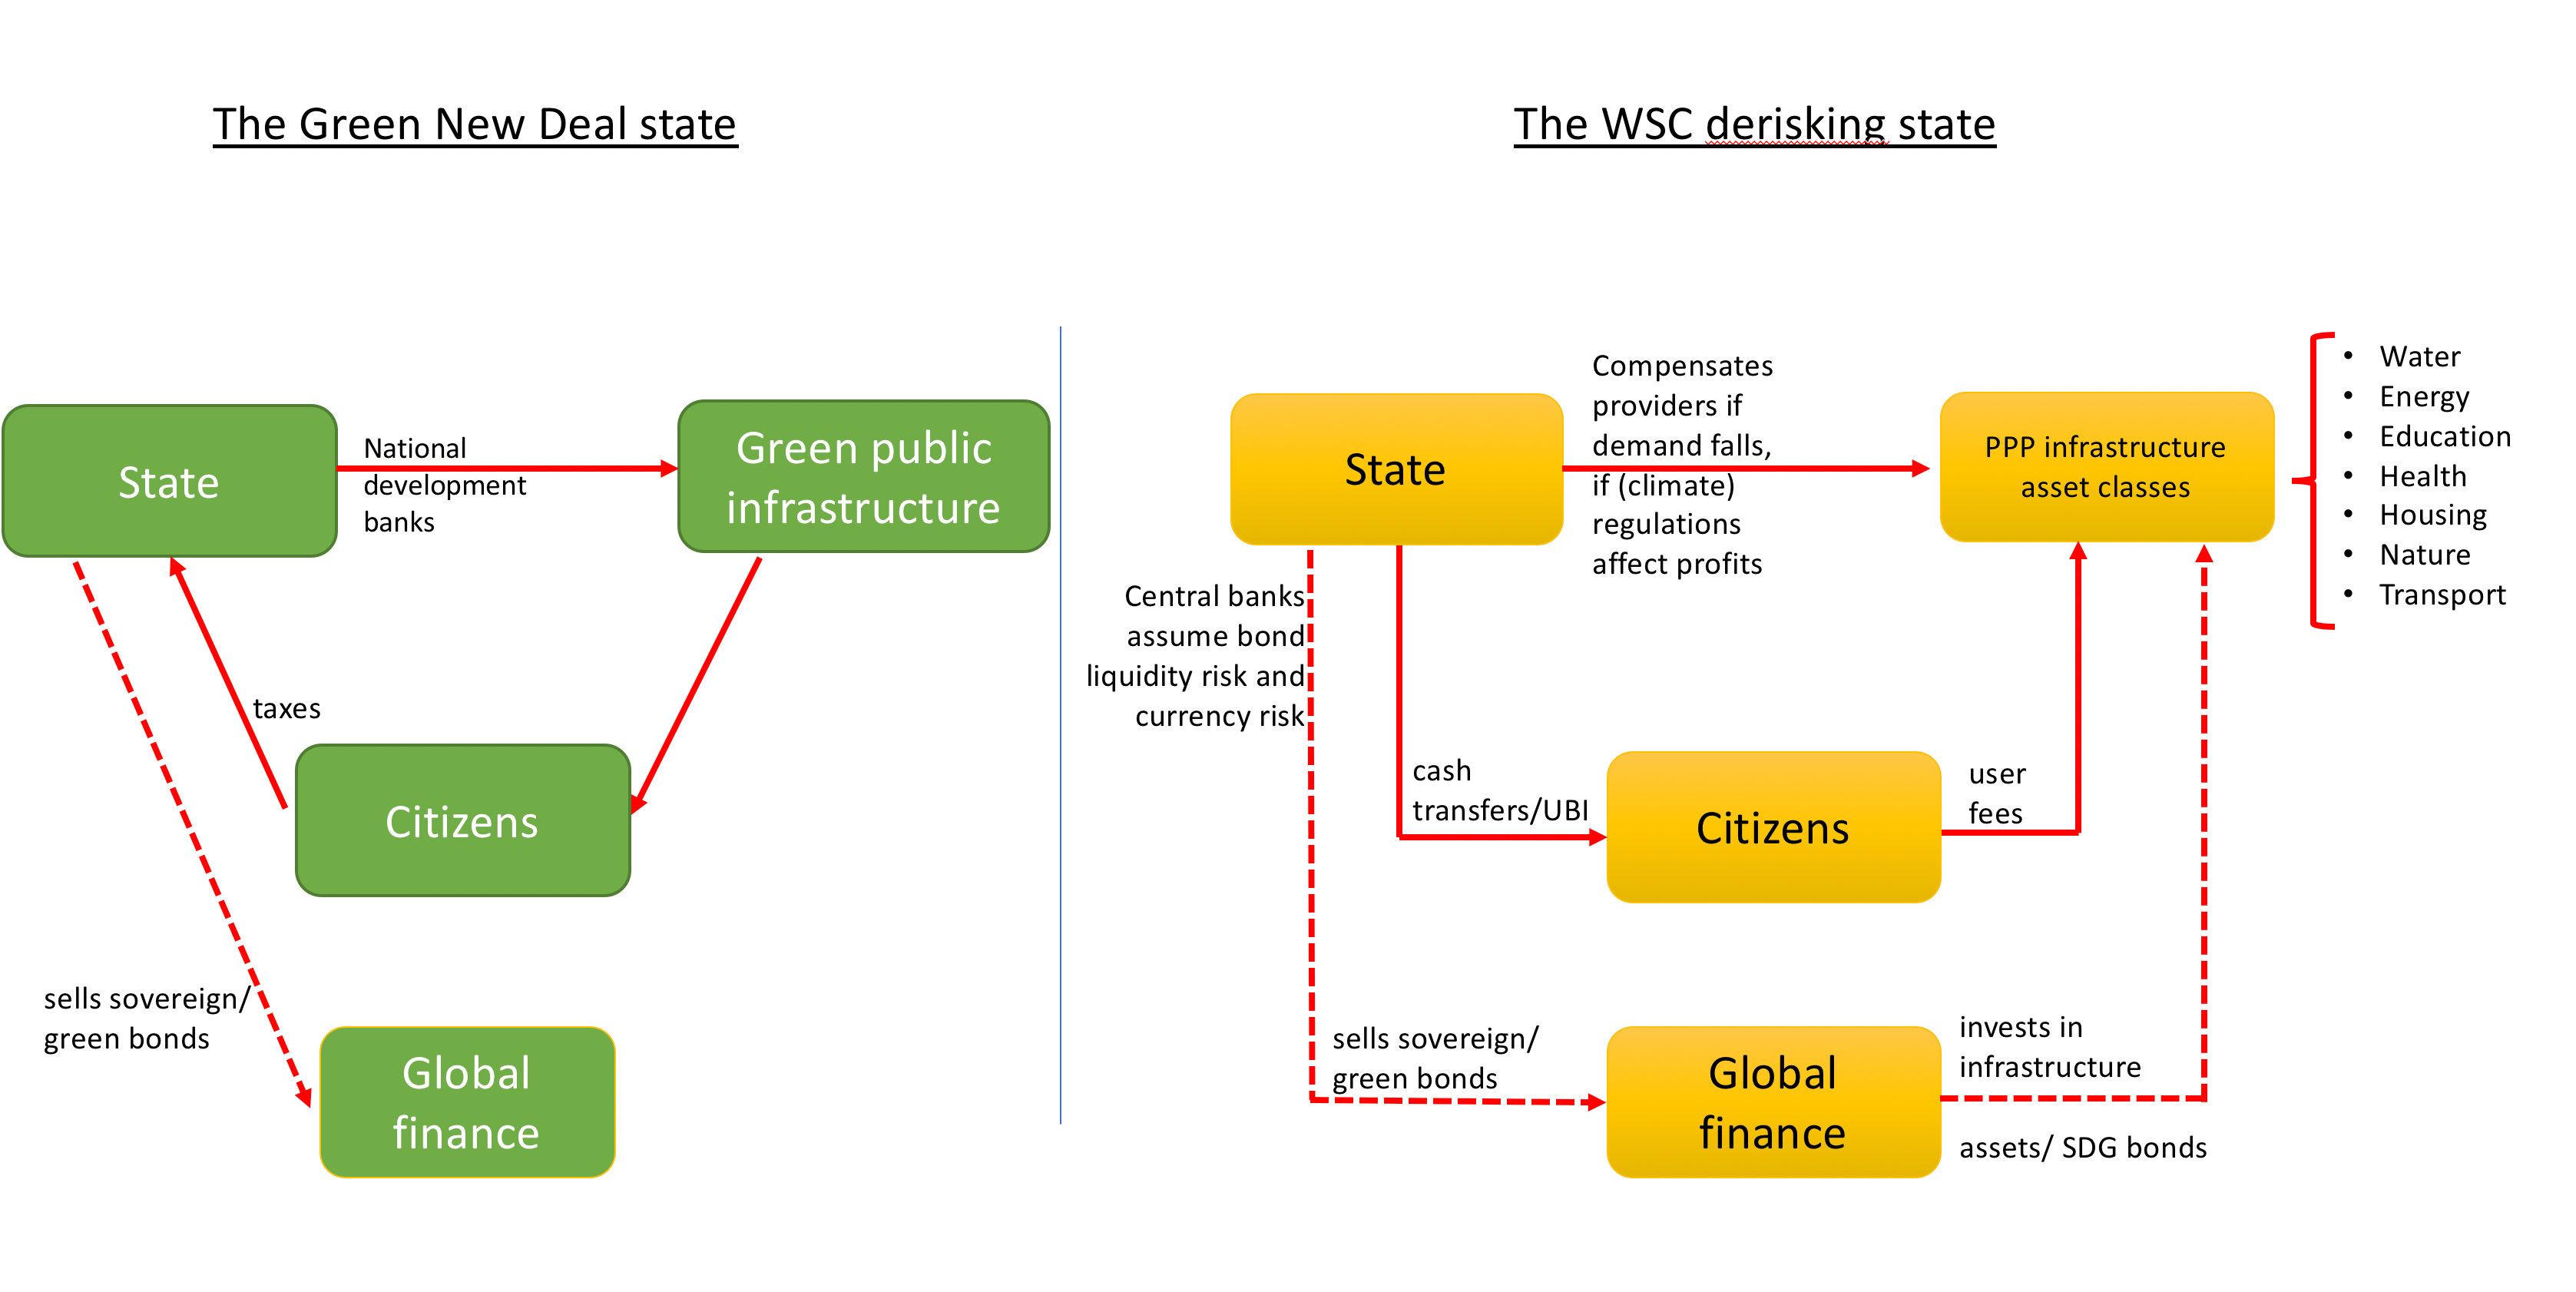
\includegraphics{fig/WSC_State.png}

In the derisking mode of governance, the state designs a menu of sector-specific policy
and financial derisking measures to encourage PPPs, accepts that this involves the
commodification of infrastructure via user-fees but puts in place cash
transfers/universal basic income schemes to mitigate the potential exclusion of the poor
from these services. That the derisking state does distributional politics through cash
transfers paradoxically accommodates calls for rethinking welfare politics as wage
labour becomes increasingly precarious.
Cash transfers enable the poor to access commodified public services,
and where these are not large enough, the state steps in to guarantee cash flows to investors.

Thus, development is not simply one-side defined by the political economy of capital,
but more specifically, by financial capital seeking to expand to new
areas, for which it colonises the infrastructure of the state. Financial capital no longer
just drags the poor into the embrace of the market, but also the state.

The derisking state can thus be understood as a project that seeks to extend the
infrastructural dependence of the state on finance -- and thus the infrastructural power
of the latter -- from its two traditional domains of monetary and fiscal policy to other
arenas of the government.

Derisking is not just about the transfers of risks to the state.
It is also about exercising infrastructural power to prevent
(regulatory) risks from materialising.

Derisking involves the central bank taking on its balance sheet bond liquidity and
currency market risks.

The legal battles to code capital into development asset
classes requires the state to take risks from the private sector onto its balance sheet, in
a clandestine reorienting of public resources that maintains the ideological commitment
to `fiscal responsibility'.

The WSC state assumes demand risk in user-fee based (social) infrastructure and
political risk that future governments might (re-)nationalize commodified
infrastructure or introduce tighter regulations, ranging from labour laws to climate
regulations that would affect profitability.

Uruguay's PPP law, passed by the
Mujica government in 2011, caps the total direct and contingent liabilities generated by
PPPs for the state to 7\% of the previous year's GDP, and fiscal transfers to private
operators to 0.5\% of previous year's GDP.

The fiscal costs of protecting investors from demand volatility will rise rapidly as
extreme climate events accelerate. Indeed, the climate crisis creates political and
demand risks that institutional investors need de-risking for.

The WSC protects investors against the political risks associated with green
developmental states. The green developmental state would prioritise the reorientation
of finance towards low-carbon activities. This requires a public taxonomy of green/dirty
assets that overcomes the shortcomings of private ESG ratings, and policies to penalize
dirty assets (through capital requirements or haircuts) 21 . Yet in the Wall Street
Consensus framework, such policies would classify as political risks, and require the
state to compensate their holders.

In its strategy to mutate climate risks into political and demand risks, private finance
may have found an important ally. Central banks conceptualize the immediate impact
of tighter climate rules regulation that increase the cost of funding or dramatically
change asset values as \emph{transition risks}.
The faster the low-carbon
transition, it is argued, the higher the potential that transition risks affect financial
stability, thus binding central banks in political trade-offs that privilege incremental
green regulatory regimes and accommodate greenwahing, however urgent the climate
crisis. Indeed, when central banks prioritize transition risks, they effectively rely on
private finance to drive the climate agenda, with their coordinating role focused on
subsidizing green assets, via so-called `green quantitative easing'.

In seeking to enlist central banks in the political coalitions against biting climate
regulation, the Wall Street Consensus constrains the green developmental states
directly, by making it liable for transition risks that can be framed as political and
demand risks, and indirectly, by reducing the public resources and central bank support
for Green New Deal programs that can effectively manage transition risks. The de-
risking state and the green developmental state can hardly co-exist, particularly within
market-based financial structures.

\textbf{Derisking market-based finance (formerly known as shadow banking)}

The turn to private finance as vehicle for sustainable development requires a change in
financial structures to accommodate the portfolio glut. It makes shadow banking,
understood as the production (via securitization) and financing (via wholesale funding
and derivative markets) of tradable securities, the desirable structure for financial
systems across the Global South. Indeed, the WSC consolidates
several global initiatives to restructure bank-based financial systems into market-based
finance or shadow banking,
where institutional investors can easily purchase local bonds (securities), including
infrastructure-backed securities, and finance as well as hedge their securities positions
via repos and derivative markets. Structural policies shift from developmental states'
concern with the productive structure, to the financial system.

The Financial Stability Board announced in 2015 that its new priority would be to transform
shadow banking into resilient market-based finance, which it defined as securities,
derivatives and repo markets.

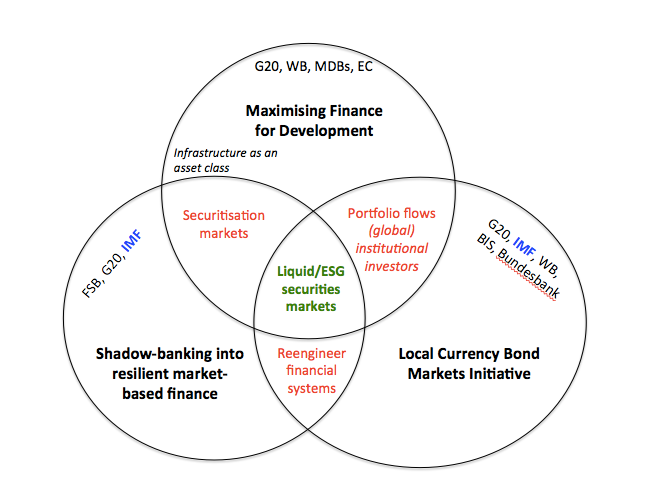
\includegraphics{fig/new_development_finance.png}

Figure: The turn to securities markets/market-based finance in international development

In sum, the organizational promoters of the Wall Street
Consensus championed in a multiplicity of global regulatory spaces the idea that
financial structure change is critical to attract the portfolio glut.

The
securitization of infrastructure loans would create both highly rated, low-return
tranches suitable for conservative pension funds/asset managers and lower-rated,
higher return tranches suitable for risk-driven investors. It would also accelerate lending
to infrastructure projects, constrained by Basel III rules for banks.

Since market-based finance is more systemically vulnerable than traditional bank-based
systems, the Wall Street Consensus assigns a triple de-risking role to central banks: in
bond markets and currency markets as market-makers of last resort,
and, forced by the inevitable consequences of green washing, as climate rescuers of last
resort, for assets left devalued by extreme climate events.
Some derisking
interventions, particularly in government bond markets, are at odds with the ideological
premises of central bank independence. Thus, the process of implicating central banks
in upholding the institutional basis of the derisking-centred accumulation regime is
incremental. It builds on crises such as the COVID19 pandemic to normalize new
derisking practices.

Greenwashing, like any
other regulatory arbitrage, eventually confronts its architects with the systemic
problems it feeds -- extreme climate events will devalue carbon-intensive assets and
greenwashed assets. The political logic of the Wall Street Consensus calls for central
banks to rescue the holders of last resort for carbon-intensive assets (Jahnke, 2019), to
risk-proof their portfolios, taking on its balance sheet the consequences of systemic
greenwashing.

`Development aid is dead, long-live private finance!'

\emph{Conclusion}

The Wall Street Consensus re-imagines international development interventions as
opportunities for global finance. In the new `development as derisking' paradigm,
institutional investors and asset managers are able to influence, if not altogether shape,
the terms on which poor countries join the global supply of `SDG' securities.
Multilateral development banks lead the efforts to design the ``de-risking''/subsidies
measures that seek to protect global investors from political risk or the demand risk
associated with privatized public services.

Equally important, this is a state-building project that puts in place the institutional
basis for a new regime of derisking as accumulation. The state comes under pressure
to institutionally codify risk-proofing arrangements, guaranteeing private financial
profits in the name of aligning sustainable projects with the preferred risk/return profile
of institutional investors. This includes adopting the US model of private pensions and
insurance to create local institutional investors. The tendency toward concentration in
the asset management sector (to exploit economies of scale and scope) may result in
Global North asset managers absorbing the funds of poor countries' institutional
investors and making allocative decisions on a global level.

In pushing for financial system change, development as derisking threatens to render
obsolete the old developmental banking model that put finance in the service of well-
designed industrial strategies. Development banks join the efforts of constructing and
derisking development asset classes. This is a political choice. Developmental banking
can arguably better serve a sustainability agenda because banks can easier include,
monitor and enforce safeguard policies in long-term relationships with customers. Most
countries with a successful experience of industrialisation relied on public development
banking as a critical pillar of industrial policies (Naqvi et al, 2018). Public development
banking allowed the developmental state to derisk via long-term loans to industrial
sectors identified as strategic by an industrial policy aimed at promoting the
international competitiveness of local firms.

This re-engineering of financial systems in the Global South, threatens the space for
alternative development strategies, and for a green developmental state. Government
capacity to design autonomous policies, in many poor countries severely eroded by
structural adjustment, will be further eroded by pressures to allocate scarce resources
to creating the conditions for private development finance.

\href{https://onlinelibrary.wiley.com/doi/abs/10.1111/dech.12645}{Daniela Gabor (2021) The Wall Street Consensus (Paywall)}
\href{pdf/Gabor_2021_Wall_Street_Consensus.pdf}{Draft (pdf)}

\hypertarget{part-appendices}{%
\part{Appendices}\label{part-appendices}}

\hypertarget{appendix-appendices}{%
\appendix}


\hypertarget{about}{%
\chapter{About}\label{about}}


\includegraphics{fig/me.jpg}

\emph{Dyre Haugen} and \emph{Dyrehaugen} is Webian for \emph{Jon Martin} -
self-owned Globian, Webian, Norwegian and Canarian with
a background from industrial research policy, urban planning and
economic development consulting on global, regional and urban scales.
I am deeply concerned about the (insane) way
humanity (i.e.~capitalism) interfere with nature.
In an effort to gain insights in how and why this happens
stuff is collected from around the web and put together
in a linked set of web-sites.
The sites are operated as personal notebooks.
However, these days things can be easily published to the
benefit of others concerned with the same issues.
But be aware - this is not polished for presentation or
peer-reviewed for exactness.
I offer you just to have a look at my `work-desk' as it appears in the moment.
Any comment or suggestion can be mailed to \href{mailto:dyrehaugen@gmail.com}{\nolinkurl{dyrehaugen@gmail.com}}
You can follow me on twitter as @dyrehaugen.
Thanks for visiting!

\hypertarget{links}{%
\chapter{Links}\label{links}}

\textbf{Current Dyrehaugen Sites:}

\begin{itemize}
\tightlist
\item
  \href{https://dyrehaugen.github.io/rcap}{rcap - On Capitalism} \href{http://localhost/rcap}{(loc)}
\item
  \href{https://dyrehaugen.github.io/rclm}{rclm - On Climate Change} \href{http://localhost/rclm}{(loc)}
\item
  \href{https://dyrehaugen.github.io/recs}{recs - On Economics} \href{http://localhost/recs}{(loc)}
\item
  \href{https://dyrehaugen.github.io/rngy}{rfin - On Finance} \href{http://localhost/rfin}{(loc)}
\item
  \href{https://dyrehaugen.github.io/rngy}{rngy - On Energy} \href{http://localhost/rngy}{(loc)}
\item
  \href{https://dyrehaugen.github.io/renv}{renv - On Environment} \href{http://localhost/renv}{(loc)}
\item
  \href{https://dyrehaugen.github.io/rsts}{rsts - On Statistics} \href{http://localhost/rsts}{(loc)}
\item
  \href{https://dyrehaugen.github.io/rurb}{rurb - On Urbanization} \href{http://localhost/rurb}{(loc)}
\item
  \href{https://dyrehaugen.github.io/rvar}{rvar - On Varia} \href{http://localhost/rvar}{(loc)}
\item
  \href{https://dyrehaugen.github.io/rwsd}{rwsd - On Wisdom} \href{http://localhost/rwsd}{(loc)}
\end{itemize}

\textbf{Blogs:}

\begin{itemize}
\tightlist
\item
  \href{https://dyrehaugen.github.io/rde}{rde - Blog in English} \href{http://localhost/rde}{(loc)}
\item
  \href{https://dyrehaugen.github.io/rdn}{rdn - Blog in Norwegian} \href{http://localhost/rdn}{(loc)}
\end{itemize}

\textbf{Discontinued:}

\begin{itemize}
\tightlist
\item
  \href{https://dyrehaugen.github.io/jdt}{jdt - Collection (Jekyll)} \href{http://localhost/jdt}{(loc)}
\item
  \href{https://dyrehaugen.github.io/hdt}{hdt - Collection (Hugo)} \href{http://localhost/hdt}{(loc)}
\end{itemize}

\textbf{Not listed:}

\begin{itemize}
\tightlist
\item
  (q:) dhe dhn jrw56
\item
  (z:) rcsa rpad rstart
\end{itemize}

\hypertarget{news}{%
\chapter{NEWS}\label{news}}

\hypertarget{gfanz-low-carbon-banking}{%
\section{210421 GFANZ: Low Carbon Banking}\label{gfanz-low-carbon-banking}}

Banks and financial institutions with more than \$70tn assets have pledged to cut their greenhouse gas emissions and ensure their investment portfolios align with the science on the climate.

In the initiative, chaired by Mark Carney, the former governor of the Bank of England, 160 companies, including 43 banks from 23 countries, will set targets to cut the carbon content of their assets by 2030, in line with an overall goal of net zero emissions by 2050.

The forum, the \emph{Glasgow Financial Alliance for Net Zero}, aims to encourage the financial sector to divert investment towards low-carbon infrastructure and technologies, and to discourage high-carbon investments, ahead of Cop26, the vital UN climate talks to be hosted by the UK in Glasgow this November.

Janet Yellen, the US Treasury secretary, and John Kerry, the US special presidential envoy for climate, are backing the alliance.

GFANZ {[}will be{]} the gold standard for net zero commitments in the financial sector.
The alliance would not allow banks to ``greenwash'' their commitments.

However, since the signing of the Paris agreement in 2015 banks have poured at least
\href{https://www.theguardian.com/environment/2021/mar/24/big-banks-trillion-dollar-finance-for-fossil-fuels-shocking-says-report}{\$3.8tn into fossil fuel financing}.

The financial system is fuelling environmental breakdown on a catastrophic scale, and what we really need is for central banks to play their roles as regulators and take concrete action to prevent all of the firms they oversee from making investments that are incompatible with governments' climate targets.

Banks signing up to GFANZ would be required to show ``credible plans'' for reducing their investment in high-carbon assets, but would not face a deadline for exiting fossil fuel investment.
Advertisement

Officials said there would be no blanket requirements for companies to stop financing coal, for instance, and banks would be allowed to make their own judgments on the carbon content of their portfolios, on a case by case basis.

\href{https://www.theguardian.com/business/2021/apr/21/leading-finance-firms-sign-up-to-mark-carney-forum-on-low-carbon-investment}{Guardian}

  \bibliography{book.bib,packages.bib}

\end{document}
